\documentclass[11pt,a4paper]{article}
\usepackage[T1]{fontenc}
\usepackage[utf8]{inputenc}
\usepackage{amsmath,amsthm}
\usepackage{newpxtext,newpxmath}
\usepackage[defaultsans]{lato}
\usepackage{inconsolata}
\usepackage[a4paper,top=24mm,bottom=23mm,left=24mm,right=24mm,headsep=9mm]{geometry}
\usepackage{microtype,mathtools,bm,graphicx,booktabs,longtable,tabularx,array}
\usepackage[table]{xcolor}
\usepackage{tikz}
\usetikzlibrary{arrows.meta,positioning,calc,fit,backgrounds}
\usepackage[most]{tcolorbox}
\usepackage{fancyhdr,titlesec,enumitem,caption,float,needspace,listings,url}
\usepackage[unicode,pdfencoding=auto]{hyperref}
\definecolor{navy}{HTML}{102E3A}
\definecolor{teal}{HTML}{107B80}
\definecolor{slate}{HTML}{586B73}
\definecolor{pale}{HTML}{F0F5F5}
\definecolor{gold}{HTML}{B59555}
\definecolor{rulegray}{HTML}{D3DFE1}
\hypersetup{colorlinks=true,linkcolor=navy,urlcolor=teal,citecolor=teal,
 pdftitle={Tom Klootwijk - Unified Field Theory V2: UU ID},
 pdfauthor={Tom Klootwijk},
 pdfsubject={UU ID, Agnostic Boundary Horizon and chronotemporal identity},
 pdfkeywords={Tom Klootwijk, UU ID, Double Set Operator, Agnostic Boundary Horizon, Theseus, Unified Field Theory V2}}
\AtBeginDocument{\fontsize{10.5}{13}\selectfont
 \setlength{\abovedisplayskip}{7pt plus 2pt minus 2pt}
 \setlength{\belowdisplayskip}{7pt plus 2pt minus 2pt}
 \setlength{\abovedisplayshortskip}{3pt plus 2pt}
 \setlength{\belowdisplayshortskip}{5pt plus 2pt minus 2pt}}
\setlength{\parindent}{0pt}
\setlength{\parskip}{5pt}
\setlength{\emergencystretch}{2em}
\setlength{\headheight}{15pt}
\setlength{\tabcolsep}{5pt}
\renewcommand{\arraystretch}{1.12}
\setlist{nosep,leftmargin=1.5em,topsep=4pt}
\setcounter{tocdepth}{1}
\numberwithin{equation}{section}
\captionsetup{font=small,labelfont={bf,sf},labelsep=period,skip=7pt}
\titleformat{\section}{\sffamily\LARGE\bfseries\color{navy}}{\thesection}{.65em}{}
\titleformat{\subsection}{\sffamily\large\bfseries\color{teal}}{\thesubsection}{.6em}{}
\titleformat{\subsubsection}{\sffamily\normalsize\bfseries\color{navy}}{\thesubsubsection}{.6em}{}
\titlespacing*{\section}{0pt}{0pt}{14pt}
\titlespacing*{\subsection}{0pt}{13pt}{5pt}
\titlespacing*{\subsubsection}{0pt}{10pt}{4pt}
\pagestyle{fancy}\fancyhf{}
\fancyhead[L]{\sffamily\scriptsize\color{slate}TOM KLOOTWIJK}
\fancyhead[R]{\sffamily\scriptsize\color{slate}UNIFIED FIELD THEORY V2 / UU ID}
\fancyfoot[L]{\sffamily\scriptsize\color{slate}FORMAL CORPUS EDITION 2.0}
\fancyfoot[R]{\sffamily\small\color{navy}\thepage}
\renewcommand{\headrulewidth}{.3pt}
\newcommand{\newsec}[1]{\clearpage\section{#1}}
\newcommand{\src}[2]{{\sffamily\small\color{slate}[#1, #2]}}
\newcommand{\origin}[1]{{\sffamily\small\color{slate}#1}\par\vspace{3pt}}
\newcommand{\uu}{\operatorname{UU\,ID}}
\newcommand{\dcup}{\mathbin{\cup\!\cup}}
\newcommand{\ind}{\mathbf 1}
\newcommand{\dist}{\operatorname{dist}}
\newcommand{\clip}{\operatorname{clip}}
\newcommand{\trunc}{\operatorname{trunc}_0}
\newcommand{\pop}{\operatorname{popcount}}
\newcommand{\val}{\operatorname{value}}
\newcommand{\xor}{\mathbin{\oplus}}
\newcommand{\cat}{\mathbin{\Vert}}
\newcommand{\dd}{\mathrm d}
\newtcolorbox{formal}[1]{enhanced,breakable,colback=pale,colframe=teal,boxrule=.55pt,sharp corners,left=10pt,right=10pt,top=8pt,bottom=8pt,coltitle=white,colbacktitle=teal,fonttitle=\sffamily\bfseries,title={#1},before skip=9pt,after skip=9pt}
\newtcolorbox{statement}[1]{enhanced,breakable,colback=white,colframe=rulegray,boxrule=.6pt,borderline west={2pt}{0pt}{gold},sharp corners,left=11pt,right=10pt,top=8pt,bottom=8pt,fonttitle=\sffamily\bfseries,coltitle=navy,colbacktitle=pale,title={#1},before skip=9pt,after skip=9pt}
\lstset{basicstyle=\ttfamily\small,breaklines=true,columns=fullflexible,keepspaces=true,frame=single,rulecolor=\color{rulegray},backgroundcolor=\color{pale},xleftmargin=5pt,xrightmargin=5pt,aboveskip=8pt,belowskip=8pt,showstringspaces=false}
\begin{document}
\hypersetup{pageanchor=false}
\begin{titlepage}\thispagestyle{empty}
\begin{tikzpicture}[remember picture,overlay]
\fill[navy] (current page.north west) rectangle (current page.south east);
\fill[teal] ($(current page.north west)+(0,-18mm)$) rectangle ($(current page.north east)+(0,-21mm)$);
\draw[gold,line width=.6pt] ($(current page.south west)+(24mm,44mm)$)--($(current page.south east)+(-24mm,44mm)$);
\end{tikzpicture}
\color{white}\vspace*{12mm}
{\sffamily\small OPEN NOTATION\quad /\quad CHRONOTEMPORAL IDENTITY\par}
\vspace{24mm}
{\sffamily\fontsize{29}{34}\selectfont TOM KLOOTWIJK\par}
\vspace{5mm}
{\sffamily\fontsize{12}{17}\selectfont NL200678942\quad /\quad 10-07-1990\par}
\vspace{16mm}
{\sffamily\bfseries\fontsize{44}{49}\selectfont UNIFIED\par FIELD THEORY\par}
\vspace{9mm}
{\sffamily\fontsize{26}{31}\selectfont VERSION 2\quad /\quad UU ID\par}
\vspace{10mm}
{\sffamily\fontsize{14}{20}\selectfont The Double Set Operator, Agnostic Boundary Horizon,\par Theseus identity and the complete state-field wrapper\par}
\vspace{8mm}
{\fontsize{19}{25}\selectfont
\[\uu\big((d_1,T_1),(d_2,T_2)\big)
 =\min\{|d_1-T_1|,|d_2-T_2|\}.\]}
\vfill
{\sffamily\small UGTS-KC 3.6\enspace +\enspace GAMBIT 4.0\enspace +\enspace UU ID CORPUS\par}
\vspace{6mm}
{\sffamily\small FORMAL CORPUS EDITION 2.0\hfill 11 SEPTEMBER 2026\par}
\vspace{11mm}
\end{titlepage}
\hypersetup{pageanchor=true}\pagenumbering{roman}\phantomsection
\section*{Abstract}\addcontentsline{toc}{section}{Abstract}
This volume formalizes \emph{Tom Klootwijk's Unified Field Theory, Version 2}, with \emph{UU ID} as its central composition rule. The primary V2 source is the supplied 18-page document \emph{devoid the dark SDF definition where}. Its open notation compares a field value with an explicit threshold; its \emph{Agnostic Boundary Horizon} is the absolute threshold deviation; and its \emph{Double Set Operator}, also named \emph{Unsigned Union / Identity Disjunction}, selects the minimum of those deviations.

The central equation is retained exactly. V2 develops its finite-family algebra, zero sets, tolerance neighborhoods, exact unsigned-distance interpretation and label-preserving evaluation records. It formalizes the source's \emph{Chronotemporal Absorbing Field} and its \emph{Theseus Identity Field}, distinguishing the written weighted integral from the historical minimum evaluated by the source shader. Experience records, temporal connector hinges and split--merge ancestry give a precise lineage structure for the source's identity language.

The \emph{Point-Source / Genesis Horizon}, \emph{1-bit God}, \emph{Monotheistic Union} and \emph{space-as-data} vocabulary is retained as the author's named ontological postulates. Two different bit conventions in the source are carried as separate definitions: zero at the source, and zero at the threshold horizon. Their respective equations are recorded explicitly.

The retained Gambit engine supplies the operational transition, its conserved material law, bounded recurrent state, exact Boolean output and complete $118N+27$-bit encoding. V2 constructs an unsigned UU ID field for that complete word, proves an explicit decoder, and defines a conjugate next-field transition. A separate log-polar address lift preserves every cell bit and every control bit as distinct locations in a three-dimensional horizon family. The historical UU ID of state fields is shown to correspond to the bitwise OR of their complete words; the current state and the ordered lineage remain separate records.

The accompanying archive contains the editable manuscript, 36 retained operator records, 20 pattern recipes, 16 UU ID mechanisms, 34 sealed definitions, a 100-entry Dutch profile, source-variant records, schemas, Python implementations and replayable examples. The executed suite passes 126 test methods. In the declared 64-cell example, 64 direct updates and 64 unsigned-field updates agree exactly, preserve material 18,677, and emit 2,258 pulses equal to one.

\begin{statement}{Edition identity}
\textbf{Author:} Tom Klootwijk\qquad
\textbf{Identifier:} NL200678942\qquad
\textbf{Date of birth:} 10-07-1990

The same literal author record appears in the manuscript attribution, archive metadata and content-addressed example substrate. Version 2 is a complete revised corpus, with the UU ID definitions developed before the retained field-engine formalism.
\end{statement}

\clearpage\tableofcontents\clearpage\pagenumbering{arabic}
\section{Author, corpus and the V2 identity object}
\label{sec:author}
\origin{Primary V2 basis: S3, physical pp. 1--18. Retained substrate: S1. Retained engine: S2.}

\subsection{Attribution and the meaning of UU ID}
The literal author record is
\begin{equation}
\mathsf a_{\rm TK}=(\text{Tom Klootwijk},\ \text{NL200678942},\ \text{10-07-1990}).
\end{equation}
It is stored under the instance address \texttt{author:tom-klootwijk}. The identifier and date are retained as supplied text. They identify the documentary attribution; the field operators below have their own numerical inputs and definitions.

In the supplied source, \textbf{UU ID} means the \emph{ID Double Set Operator}, named \emph{Unsigned Union / Identity Disjunction} and written with a doubled union or parallel notation. This edition uses $\dcup$ for the composition of already normalized horizon fields, and $\uu$ when the underlying raw values and thresholds are shown. \src{S3}{pp. 2--3}

Three uses of identity are kept explicit. \emph{Documentary identity} is the author record. \emph{Definition identity} is a stable record ID together with its canonical content address. \emph{Chronotemporal identity} is the declared relationship between current state, past experience, boundary components and lineage. The scalar UU ID is one observable within that third structure.

\subsection{The source organization}
\begin{tabularx}{\textwidth}{@{}p{.11\textwidth}X@{}}
\toprule\textbf{Source} & \textbf{Organization and role in V2}\\\midrule
S3 & The primary source proceeds from open notation and UU ID (pp. 1--3), through Theseus absorption (pp. 4--6), native definitions and lineage (pp. 7--10), the Genesis and one-bit conventions (pp. 10--12), and the complete-state mapping wrapper (pp. 13--18).\\[5pt]
S1 & The retained 19-page substrate supplies the registry, geometry, topology, hinges, Dutch profile, 36 operators and 20 patterns.\\[5pt]
S2 & The retained seed, transition, U4, C1--C16 and binary encoding appear on physical pp. 4--15 of the 20-page engine document.\\
\bottomrule
\end{tabularx}

\subsection{The V2 structured identity}
The combined identity object is specified as
\begin{equation}
\mathfrak I=(\mathsf a,\mathfrak D,\sigma,S,\mathcal B,\Lambda,\mathcal I,\mathcal H).
\label{eq:identity-object}
\end{equation}
Here $\mathsf a$ is the attribution record; $\mathfrak D$ is the definition registry; $\sigma$ is a complete numerical seed; $S$ is its current operative state; $\mathcal B$ is the labelled boundary family; $\Lambda$ is committed lineage; $\mathcal I$ is the retained integral observable; and $\mathcal H$ is the historical horizon observable. This tuple is a V2 construction connecting the source's named components. An instance may declare only the components relevant to its pipeline.

The edition's author instance supplies $\mathsf a_{\rm TK}$. The numerical and experience examples supply their own explicit synthetic records; no personal experience history is inferred from the attribution tuple. Field and lineage identities are evaluated from their actual supplied records.

\textbf{Source conventions.} Source formulas and implementation sketches retain their stated meanings. New executable bindings are marked as V2 constructions. Appendix~\ref{app:variants} records the integral/minimum, bit-convention, layout and decoding variants.

\newsec{Open notation and the UU ID calculus}
\label{sec:uuid}
\origin{Source definitions: S3, pp. 1--3 and 9--12. Propositions UU1--UU4: V2 derivations.}

\subsection{Raw value, threshold and relational state}
Let $X$ be a declared query domain. A boundary component has a real-valued field $d_\alpha:X\to\mathbb R$ and a threshold $T_\alpha\in\mathbb R$. For raw radial distance, $d_\alpha$ is nonnegative. More general source relations, such as the plane comparison, may use a real-valued coordinate functional. The relation is
\begin{equation}
\operatorname{rel}_\alpha(x)=
\begin{cases}
<,&d_\alpha(x)<T_\alpha,\\
=,&d_\alpha(x)=T_\alpha,\\
>,&d_\alpha(x)>T_\alpha.
\end{cases}
\end{equation}
The symbols $<$ and $>$ are order relations against a stated threshold. The open notation does not attach a moral, luminous or other interpretive polarity to them. It retains the comparison itself. This is the source's operation of removing the ``dark'' sign association. \src{S3}{pp. 1--2}

\begin{formal}{Definition UU-D1: Agnostic Boundary Horizon}
For a declared pair $(d_\alpha,T_\alpha)$, define
\[
\delta_\alpha(x)=|d_\alpha(x)-T_\alpha|,
\qquad H_\alpha=\{x:\delta_\alpha(x)=0\}.
\]
The horizon field is nonnegative. Its zero set is precisely the threshold locus $d_\alpha=T_\alpha$. Its relational state and its absolute deviation are separate outputs of the component record.
\end{formal}

For a sphere or circle, $d(x)=\|x-c\|$ and $T=r\ge0$. For a plane with unit normal $n$, $d(x)=n\cdot x$ and the threshold names the plane offset. The source's box relation uses
\begin{equation}
q(x)=\max_k(|x_k|-E_k),\qquad q(x)\lessgtr0.
\end{equation}
Each of these examples specifies a boundary relation. Its exact-distance capability is determined by the stated field and metric, rather than by the presence of a threshold alone. \src{S3}{pp. 1--2}; \src{S1}{\S4.1}

\subsection{The source's Double Set Operator}
\begin{formal}{Definition UU-D2: UU ID / Identity Disjunction}
For two boundary components,
\[
\boxed{\quad
\uu\big((d_1,T_1),(d_2,T_2)\big)(x)
=\min\{|d_1(x)-T_1|,|d_2(x)-T_2|\}.
\quad}
\]
For already normalized horizon fields, write
\[
(\delta_1\dcup\delta_2)(x)=\min\{\delta_1(x),\delta_2(x)\}.
\]
Normalization occurs once for each component. A subsequent union folds the resulting nonnegative horizon fields.
\end{formal}
This is the literal equation printed on physical page 3 and repeated on page 9 of S3. The raw field, threshold and normalized horizon remain available as individual record fields. The source shader computes two absolute differences and returns their minimum. \src{S3}{pp. 3 and 9}

\Needspace{8\baselineskip}
\begin{lstlisting}
def uu_id(d1, threshold1, d2, threshold2):
    identity1 = abs(d1 - threshold1)
    identity2 = abs(d2 - threshold2)
    return min(identity1, identity2)
\end{lstlisting}

For a finite family $A$, define
\begin{equation}
U_A(x)=\min_{\alpha\in A}\delta_\alpha(x),
\qquad U_\varnothing(x)=+\infty.
\label{eq:finite-uuid}
\end{equation}
The empty value is the mathematical identity of minimum. The executable JSON interface returns an explicit \texttt{empty} status with a null value for an empty family, so no infinite JSON number is emitted. Complete-state fields later in this volume are nonempty because they include the permanent anchor.

\subsection{UU1. The minimum algebra}
On nonnegative horizon functions, pointwise minimum is commutative, associative and idempotent:
\begin{align}
\delta_1\dcup\delta_2&=\delta_2\dcup\delta_1,\\
(\delta_1\dcup\delta_2)\dcup\delta_3
&=\delta_1\dcup(\delta_2\dcup\delta_3),\\
\delta\dcup\delta&=\delta.
\end{align}
The constant extended field $+\infty$ is an identity. These equations follow by applying the corresponding ordered-number identities at every query point. Thus the normalized fields form a meet-semilattice in their ordinary pointwise order, and a monoid after adjoining $+\infty$ as the empty-family element.

A change of grouping does not change the scalar result. The chronological order of experience absorption and the non-commutative composition of hinges are different operations; they retain their own order records. The UU ID minimum does not replace that information.

\subsection{UU2. Zero sets and identity-preservation zones}
For a nonempty finite family of nonnegative fields,
\begin{equation}
\{x:U_A(x)=0\}=\bigcup_{\alpha\in A}H_\alpha.
\label{eq:zeroset}
\end{equation}
For every $\varepsilon\ge0$,
\begin{equation}
\{x:U_A(x)\le\varepsilon\}
=\bigcup_{\alpha\in A}\{x:\delta_\alpha(x)\le\varepsilon\}.
\label{eq:tube}
\end{equation}
Both assertions follow because a finite minimum is attained: the minimum is zero, or at most $\varepsilon$, exactly when at least one component has that property. Equation~\eqref{eq:tube} gives a precise \emph{identity-preservation zone} for the source terminology.

The source table also names an \emph{Inner Core Intersect} by $(d_1<T_1)\land(d_2<T_2)$, and an \emph{Outward Disjunction} by $(d_1>T_1)\lor(d_2>T_2)$. V2 retains both predicates as relational observations. They are computed from the raw comparisons, separately from the minimum horizon value. The table's third row is incomplete in the supplied PDF; no additional equation is assigned to that row. \src{S3}{p. 3}

\subsection{UU3. Exact unsigned boundary distance}
Suppose $(X,\operatorname{d}_X)$ is a metric space and each component is exactly
\begin{equation}
\delta_\alpha(x)=\dist(x,H_\alpha).
\end{equation}
For a finite nonempty family,
\begin{equation}
U_A(x)=\dist\left(x,\bigcup_{\alpha\in A}H_\alpha\right).
\label{eq:distance-union}
\end{equation}
The distance to a finite union is the minimum of the distances to its members. In this case, each component is 1-Lipschitz, and $U_A$ is 1-Lipschitz as well. To see the latter directly, choose a minimizing component at one query point and use its Lipschitz inequality in both directions.

For the sphere field $d(x)=\|x-c\|$, the value $|d(x)-r|$ is exact distance to the sphere of radius $r$, including the point case $r=0$. A generic implicit field's absolute deviation instead has the declared residual semantics unless an exact-distance relation is established for that field.

The target set in Equation~\eqref{eq:distance-union} is the union of retained component horizons. It is not generally the boundary of the union of filled solids. For concentric radii 1 and 2, at radius 1 the UU ID is zero because the inner horizon is retained; distance to the exterior boundary of the filled union is 1. This distinction gives the source's independent boundary preservation a precise set-theoretic meaning.

\begin{figure}[H]
\centering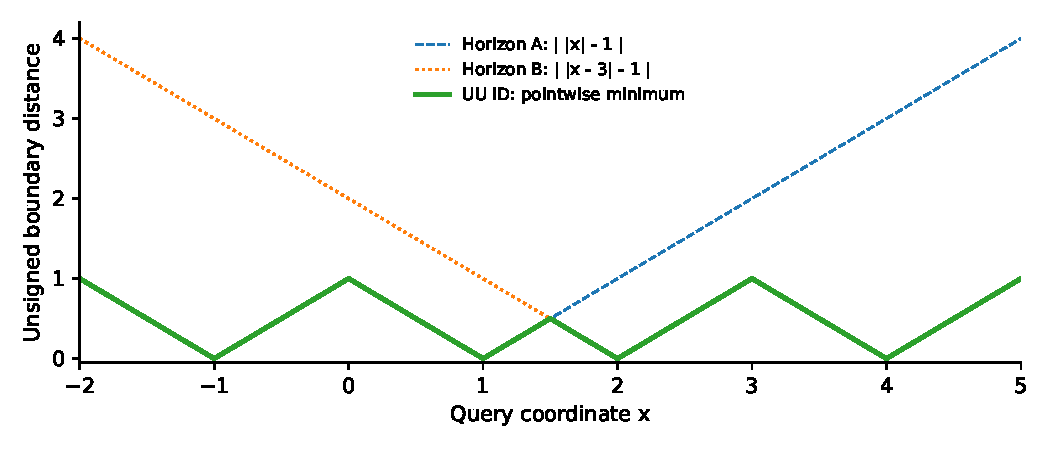
\includegraphics[width=\textwidth]{figures/uu_id.pdf}
\caption{Calculated UU ID for one-dimensional sphere horizons centered at 0 and 3, each of radius 1. The minimum retains all four component boundary points.}
\end{figure}

\subsection{UU4. Tagged composition and witness preservation}
The scalar minimum can be identical for distinct labelled families. V2 therefore defines a \emph{tagged UU ID evaluation}
\begin{equation}
\widehat U_A(x)=\big(U_A(x),\ A,\ \mathcal M_A(x),\ \mathcal R_A(x)\big),
\end{equation}
where $\mathcal M_A(x)=\{\alpha:\delta_\alpha(x)=U_A(x)\}$ is the complete set of minimizing IDs, and $\mathcal R_A(x)$ retains each raw value, threshold, relation and delta. The component definitions are retained in the associated labelled family.

Compatible families merge by ID. An ID can be repeated with the same record; different records under the same ID require a distinct versioned definition. On compatible finite maps, merge is associative, commutative and idempotent. Its scalar projection is exactly UU ID. Every input component remains retrievable, including non-minimizing components and geometrically coincident components with distinct IDs. This is V2's explicit implementation of the source's independent boundary identities.

\newsec{Genesis Horizon and the author's identity postulates}
\label{sec:genesis}
\origin{Source terminology and formulas: S3, physical pp. 10--15.}

\subsection{Point-Source / Genesis Horizon}
The source chooses a point coordinate $P_{\rm Source}$ and a structural threshold $T\ge0$. Its \emph{Genesis} field is
\begin{equation}
G(P)=\left|\|P-P_{\rm Source}\|-T\right|,
\qquad H_G=\{P:G(P)=0\}.
\label{eq:genesis}
\end{equation}
In this volume, the phrase \emph{earliest SDF definition} is retained as the source's foundational-order designation for this primitive. The formula has a complete mathematical signature once the coordinate domain, its norm and the threshold are declared. In a Euclidean domain it is the exact unsigned distance to the sphere about $P_{\rm Source}$, or to the source point when $T=0$. \src{S3}{pp. 10--12}

The supplied JSON declares a four-coordinate source point and threshold 1. Its role is preserved in the literal node \texttt{uu2:genesis}. A three-coordinate or one-coordinate instance is a separately declared specialization of the same point-source construction.

\subsection{Two named one-bit conventions}
The prose and JSON in S3 use different zero loci. V2 records both:
\begin{align}
b_{\rm source}(P)&=\ind\{\|P-P_{\rm Source}\|>0\},\\
b_{\rm horizon}(P)&=\ind\{\|P-P_{\rm Source}\|\ne T\}
                 =\ind\{G(P)>0\}.
\end{align}
The first gives zero at the source and one away from it, matching the source's ``Singular Unmanifest Source / Manifest Field'' description. The second gives zero on the threshold horizon and one away from it, matching the explicit \texttt{bit\_state} expression in the JSON. For $T>0$, the two functions differ at both the source and the horizon. \src{S3}{pp. 10--12}

A computational tolerance has an explicit field:
\begin{equation}
b_{{\rm horizon},\varepsilon}(P)=\ind\{G(P)>\varepsilon\},\qquad\varepsilon\ge0.
\end{equation}
At $\varepsilon=0$, this is the exact source equation. A positive value defines a horizon neighborhood rather than silently changing equality into an approximate test.

\subsection{Named ontological postulates}
\begin{statement}{P1. The 1-bit God / source postulate}
The source names the point-source identity and its manifestation relation the \emph{1-bit God}. Within the author's ontology, the bit marks the stated source/manifestation or horizon/off-horizon distinction. The chosen bit convention is recorded with the definition.
\end{statement}
\begin{statement}{P2. Monotheistic Union}
The source interprets a shared field of origin and its retained horizon variations as \emph{Monotheistic Union}. Its specified mathematical composition is UU ID over the declared family of origin, structural and experiential horizons.
\end{statement}
\begin{statement}{P3. Space-as-data and Theseus identity}
The source assigns identity to a chronotemporal history of structural and experiential transitions and interprets the state-as-geometry construction as \emph{space is data}. V2 retains this as an authorial identity postulate, alongside the explicit encoding, decoding and lineage maps that formalize its computational relations.
\end{statement}
These statements preserve the source's spiritual and ontological vocabulary. The mathematical theorems in later sections identify the operators, domains and hypotheses used in their proofs. The personal author record, the source-point parameter and an operative output bit remain separately named objects in the formal signature.

\subsection{The Genesis--Theseus composition}
Writing the Theseus observable as $\mathcal S_T(P)$ with its own threshold $T_T$, the source's composition is
\begin{equation}
U_{G,T}(P)=\min\left\{
\left|\|P-P_{\rm Source}\|-T_G\right|,
\left|\mathcal S_T(P)-T_T\right|
\right\}.
\end{equation}
The threshold $T_T$ has the units and codomain appropriate to the declared Theseus observable. If that observable is an accumulated integral, the second term is its threshold residual. If it is an exact geometric boundary distance, its corresponding metric capability is recorded explicitly. These are two typed instantiations of the same source formula. \src{S3}{pp. 11--12}

A common scalar composition does not by itself specify geometric connectedness. For a finite family of connected nonempty horizon neighborhoods whose intersection graph is connected, their union is connected: order the components along a spanning tree and add each one through a nonempty intersection. This is an explicit geometric condition for an unbroken neighborhood. The lineage condition for an unbroken \emph{identity history} is instead the parent-path condition in Section~\ref{sec:theseus}.

\newsec{Theseus identity and chronotemporal absorption}
\label{sec:theseus}
\origin{Source formulas: S3, pp. 4--6. Lineage and temporal hinges: pp. 7--10.}

\subsection{The source's Chronotemporal Absorbing Field}
The supplied source writes its identity field as an integral of experienced knowledge weighted by temporal retention:
\begin{equation}
\mathcal S_T(P)=\int_0^t\mathcal D(P,E(\tau))e^{-\lambda(t-\tau)}\,\dd\tau.
\label{eq:source-integral}
\end{equation}
$E(\tau)$ is the experienced knowledge/material state, $\mathcal D$ is the stated spatial/conceptual distance, and $\lambda$ is the decay or retention coefficient. The source allows $P=(x,y,z,t)$. \src{S3}{pp. 4--5}

V2 makes the analytic signature explicit. A declared query space $\mathsf P$, experience space $\mathsf E$ and comparison function
\begin{equation}
\mathcal D:\mathsf P\times\mathsf E\longrightarrow[0,\infty)
\end{equation}
are required. For each query $P$, the integrand is measurable and integrable on the stated finite interval, and $\lambda\ge0$. A shared metric can be supplied through an explicit common-coordinate representation. The source does not give a complete metric for arbitrary experience tensors; that map is a parameter of a concrete identity instance.

To keep the query argument separate from the integration endpoint, define the V2 notation
\begin{equation}
\mathcal I(P,t)=\int_0^t\mathcal D(P,E(\tau))e^{-\lambda(t-\tau)}\,\dd\tau.
\end{equation}
Equation~\eqref{eq:source-integral} is recovered by evaluating this function at the source's declared $P$, including a time-dependent query when that is part of the instance. This notation does not replace the source integral; it makes its evaluation arguments explicit.

\subsection{UU5. Exact segment recurrence at a fixed query}
For a fixed $P$ and $t_{n+1}=t_n+\Delta t$, split the integral at $t_n$:
\begin{equation}
\mathcal I(P,t_{n+1})=e^{-\lambda\Delta t}\mathcal I(P,t_n)
+\int_{t_n}^{t_{n+1}}\mathcal D(P,E(\tau))e^{-\lambda(t_{n+1}-\tau)}\,\dd\tau.
\label{eq:integral-split}
\end{equation}
In the explicit V2 piecewise-constant profile, $\mathcal D(P,E(\tau))=v_n$ on the new segment. Then
\begin{equation}
I_{n+1}=e^{-\lambda\Delta t}I_n+g_\lambda(\Delta t)v_n,
\qquad
 g_\lambda(s)=\begin{cases}
(1-e^{-\lambda s})/\lambda,&\lambda>0,\\
s,&\lambda=0.
\end{cases}
\label{eq:integral-update}
\end{equation}
This is exact for the declared segment profile. The code evaluates the numerator with \texttt{expm1} to retain small-argument precision. With $v_n\ge0$, the update preserves nonnegativity. Segment composition follows directly from Equation~\eqref{eq:integral-split}.

For $\lambda>0$, equal-duration absorptions generally depend on order. Applying values $a$ then $b$ yields $g_\lambda(s)(e^{-\lambda s}a+b)$ from zero memory, while the reverse gives $g_\lambda(s)(e^{-\lambda s}b+a)$. Their difference is nonzero when $a\ne b$. This gives the temporal connector chain a concrete non-commutative absorption example.

If the query moves, recomputing the integral at $P(t)$ is a different calculation. Under differentiability assumptions, the derivative includes both the endpoint/retention term and the query-motion term:
\begin{equation}
\frac{\dd}{\dd t}\mathcal I(P(t),t)
=\mathcal D(P(t),E(t))-\lambda\mathcal I(P(t),t)
+\dot P(t)\cdot\nabla_P\mathcal I(P(t),t).
\end{equation}
The simple segment recurrence above uses a fixed query and the declared segment values. A moving-query instance must supply its own comparison values or this additional transport information.

\subsection{The historical UU ID envelope}
The source shader on page 6 computes a different observable. It takes the minimum over the absolute deviation of each retained historical boundary:
\begin{equation}
\mathcal H(P,t)=\min_{\alpha:\,\tau_\alpha\le t}
\left|d_\alpha(P)-T_\alpha\right|.
\label{eq:history-envelope}
\end{equation}
There is no exponential factor in that shader and no summation of the layers. V2 retains this as the \emph{historical UU ID envelope}, alongside the weighted absorbing field rather than substituting one for the other. \src{S3}{pp. 5--6}

With a growing finite history at a fixed query, $\mathcal H(P,t)$ is nonincreasing. Appending a layer gives
\begin{equation}
\mathcal H_{n+1}(P)=\min\{\mathcal H_n(P),\delta_{n+1}(P)\}.
\end{equation}
The scalar result is order-independent and idempotent in its layer family. The labelled history and temporal integral retain information that this scalar minimum does not contain. A continuous-index version uses an infimum; it becomes a minimum when the relevant history parameter set is compact and its deviation function is continuous.

\begin{tabularx}{\textwidth}{@{}p{.25\textwidth}X X@{}}
\toprule\textbf{Property} & \textbf{Absorbing integral $\mathcal I$} & \textbf{Historical envelope $\mathcal H$}\\\midrule
Operation & Retention-weighted accumulation. & Minimum threshold deviation.\\
Time information & Retention weights depend on age. & Time selects admitted layers.\\
Duplicate layer & Adds a further contribution when integrated again. & Leaves the scalar minimum unchanged.\\
Empty initial value & Zero integral. & Extended value $+\infty$.\\
Units & Comparison value multiplied by time. & Units of the normalized deviation.\\
Source location & S3 pp. 4--5. & S3 pp. 5--6.\\
\bottomrule
\end{tabularx}

\subsection{The continuity threshold and the Theseus path}
The source says identity persists when the chronotemporal distance between successive states remains within $\varepsilon$. V2 writes this as a declared path condition. For states $s_0,\ldots,s_n$ in a metric space,
\begin{equation}
\operatorname{Continuous}_\varepsilon(s_0,\ldots,s_n)
\quad\Longleftrightarrow\quad
\operatorname d(s_{k-1},s_k)\le\varepsilon\quad(1\le k\le n).
\label{eq:continuity}
\end{equation}
The parent chain records which successive states constitute the path. This relation allows replacement of components while preserving a recorded chain of admitted transitions. \src{S3}{p. 5}

A bounded successive step does not assert a bounded total displacement. By the triangle inequality, $\operatorname d(s_0,s_n)\le n\varepsilon$; the endpoints need not themselves be within $\varepsilon$. For example, $0,0.75,1.5$ has consecutive distances at most 1 but endpoint distance 1.5. The persistence criterion is the recorded path, not a silent assumption that an $\varepsilon$-comparison is transitive.

\subsection{Content-addressed experience and split--merge lineage}
A V2 experience record is
\begin{equation}
\lambda_k=(\mathrm{id}_k,k,t_k,\mathrm{parents}_k,
\mathrm{parentHashes}_k,\mathrm{payload}_k,h_k).
\end{equation}
Its payload can name the boundary components, material state, comparison coordinates or knowledge record actually supplied for that experience. Every parent must already be committed. The sequence number is consecutive, timestamps are nondecreasing, and the content address covers the complete record except the hash itself. Parent addresses are included in the child record.

A split creates distinct child records referencing their parent. A merge names every retained parent. Since every edge points from an earlier committed record to a later one, induction gives an acyclic graph. The append operation preserves all existing records. Querying ancestors therefore reconstructs the explicitly recorded history of a merged identity. \src{S3}{pp. 7--10}; \src{S1}{K36-17}

\begin{figure}[H]\centering
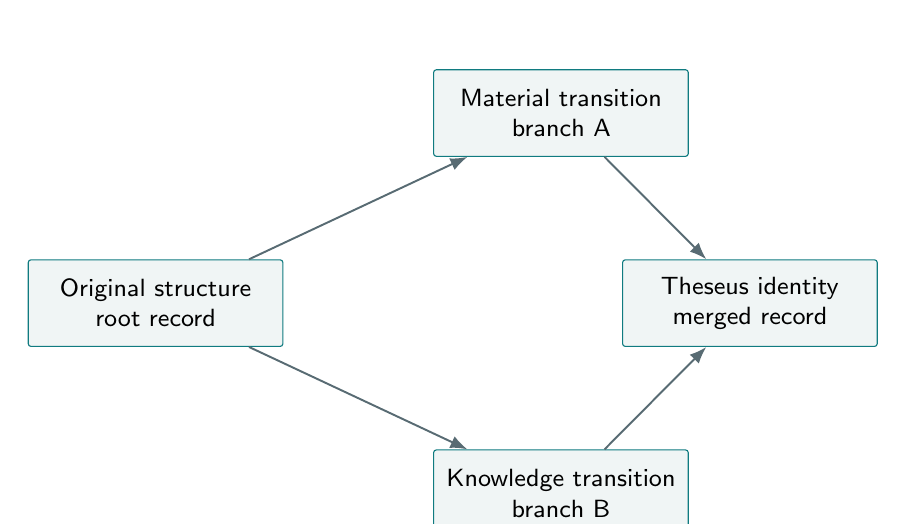
\begin{tikzpicture}[>=Latex,node distance=13mm and 19mm,
 n/.style={draw=teal,fill=pale,rounded corners=1pt,align=center,font=\sffamily\small,text width=30mm,minimum height=11mm},a/.style={->,draw=slate,line width=.7pt}]
\node[n] (root) {Original structure\\root record};
\node[n,above right=of root] (a) {Material transition\\branch A};
\node[n,below right=of root] (b) {Knowledge transition\\branch B};
\node[n,right=43mm of root] (merge) {Theseus identity\\merged record};
\draw[a] (root)--(a);\draw[a] (root)--(b);\draw[a] (a)--(merge);\draw[a] (b)--(merge);
\end{tikzpicture}
\caption{The archive's four-record synthetic split--merge example. The merge retains the content addresses of both parents.}
\end{figure}

\subsection{Temporal hinges and committed state}
The source extends the Dutch connector hinge to moments of experience and identifies a non-commutative temporal hinge chain. V2 represents a transition by the existing hinge signature
\begin{equation}
H_k=(p_k,h_k,M_k,g_k,\mathcal F_k),
\qquad M_{n:1}=M_n\circ\cdots\circ M_1.
\end{equation}
Its pivot can be a temporal connector locus, its selected map performs the declared state transformation, and its invariants record the preserved quantities. The order remains literal data. \src{S3}{p. 10}; \src{S1}{\S5}

S3 also describes continuously absorbed experience rewriting topology in real time. Its executable V2 binding names a sampling or event schedule and commits each state change as a record on that schedule. A continuous family may be evaluated between commits; the committed state and its update times are explicit. This is the specified V2 interface between the source's continuous language and its requested deterministic archive.

\newsec{Literal referential substrate and evaluation}
\label{sec:registry}
\origin{Retained basis: S1, §§3, 5 and 7. UU ID binding: S3, pp. 7--10; V2 literal registry.}

\subsection{The world and its definitions}
The retained world is
\begin{equation}
\mathcal W=(\mathfrak D,\mathcal X,\mathcal G,\mathcal R,\mathcal S,\mathcal C,
\mathcal H_g,\mathcal E,\mathcal T,\mathcal I_g,\mathcal L,\mathcal P).
\end{equation}
Its components are definitions, instances, grammar, relations, support, compatibility, hinges, events, transitions, invariants, lineage and pipelines. The subscripts on $\mathcal H_g$ and $\mathcal I_g$ distinguish the world components from the historical horizon and absorbing integral used earlier. \src{S1}{\S3.1}

A definition is a first-class record
\begin{equation}
d=(\mathrm{id},\mathrm{kind},A_d,B_d,\theta,\mathrm{Dep},p,
\mathrm{cap},\mathrm{inv},\mathrm{prov},h).
\end{equation}
It declares its domain, codomain, parameters, dependencies, evaluation phase, capabilities, invariants and provenance. The content address is
\begin{equation}
h(d)=\operatorname{SHA256}\left(\operatorname{canonicalJSON}
(d\setminus\{\mathrm{content\_hash}\})\right).
\end{equation}
The edition's canonical JSON is UTF-8 with sorted object keys, compact separators, unchanged array order and finite numerical values. The same canonicalizer is used by the registry and the experience lineage.

An instance has $(\mathrm{id},\mathrm{definition\_ref},\mathrm{literal},\mathrm{state})$. A pipeline is an ordered list of operator IDs. S3's request to make Theseus identity a native definition is realized by the same record structure used for geometry, grammar and numerical evolution. \src{S3}{pp. 7--9}

\subsection{Referential closure and deterministic resolution}
A finite registry has referential closure when IDs are unique, every dependency resolves, every content address verifies and the dependency graph is acyclic. The executable resolver repeatedly selects the lexicographically first zero-indegree node.

Every nonempty finite acyclic directed graph has a zero-indegree node. Deleting that node leaves an acyclic graph, so induction proves that the procedure visits every definition after its dependencies. The lexical tie rule fixes one deterministic resolution order. This structural order establishes availability; the stored operator pipeline separately fixes execution order.

The public interface provides \texttt{definition\_at}, \texttt{definition\_order}, \texttt{instances\_of}, \texttt{verify\_definition} and \texttt{explain\_reference}. Returned records are copies, so changing a returned value cannot mutate the registry's stored definition.

\subsection{The V2 family of 34 sealed definitions}
Eighteen retained or documentary bindings cover the author record, number literal, radix, active bits, Dutch profile, pulse projection, polygon, count comparison, connector hinge, orientation wrap, event guard, phase schedule, numerical seed, sample, edge support, transition, state word and signed C13 representation.

Sixteen UU ID bindings cover the threshold relation, absolute horizon, scalar composition, tagged composition, Genesis field, both bit conventions, absorbing integral, historical envelope, experience lineage, continuity path, unsigned complete-state horizon, decoder, relational engine hinge, layered address lift and conjugate transition. Their formal mechanism IDs are \texttt{UU2-01} through \texttt{UU2-16}. The literal definition IDs are listed in the example JSON, and every record has a computed SHA-256 content address.

The inherited \texttt{K36-07} signed-field family and \texttt{K36-08} distance capability remain named source definitions. The new UU ID family declares its nonnegative horizon codomain explicitly. The mathematical relationship between the two state representations is established through their shared complete-word encoding, rather than by giving two different operators the same unversioned definition.

\subsection{Ten-phase schedule}
\begin{center}
\begin{tabular}{@{}rlrl@{}}
\toprule\textbf{Phase} & \textbf{Operation} & \textbf{Phase} & \textbf{Operation}\\\midrule
0 & Parse literals and schemas & 5 & Evaluate support\\
1 & Normalize declared profiles & 6 & Evaluate compatibility\\
2 & Resolve and verify definitions & 7 & Evaluate or solve guards\\
3 & Construct typed objects & 8 & Commit transitions\\
4 & Apply ordered maps and hinges & 9 & Record lineage and observations\\
\bottomrule
\end{tabular}
\end{center}
The zero-based indices follow S1's phase diagram on physical page 13. A compound operator also records its internal schedule. The numerical engine's ordered stages in Section~\ref{sec:engine} are preserved inside its atomic transition. The V2 experience adapter applies its declared update at a recorded phase-8 commit and appends the resulting experience record in phase 9. \src{S1}{\S7.3}; \src{S3}{pp. 9--10}

\subsection{Support, compatibility and a boundary event}
For a declared trajectory $q(t)$ and relation $R_j$, an earliest attained admissible event is
\begin{equation}
t^*=\min\{t>t_0:R_j(q(t))=0,\ S(q(t),t)=1,\ \chi(q(t),j,t)=1,\
\mathrm{conf}\ge\mathrm{conf}_{\min}\}.
\end{equation}
The event record contains pre-state, post-state, residual, crossing direction, solver status, guard margin, route and lineage. An empty candidate family produces an explicit no-event result. An open boundary relation uses $R_j=d_j-T_j$, while its unsigned horizon uses $|R_j|$. Both have the same zero locus. Crossing direction, when required, is read from the relation or the trajectory, since the absolute value alone does not carry it. \src{S1}{\S7.2}; \src{S3}{pp. 7--8}

\newsec{The retained closed field engine}
\label{sec:engine}
\origin{Complete numerical law: S2, §§2--3, physical pp. 4--8. Relational lift: V2 construction.}

\subsection{Complete seed and finite geometry}
The complete seed is
\begin{equation}
\sigma=(\Sigma,\omega,P,I,\Theta,L,S_0,V).
\end{equation}
It contains the alphabet, ordered axiom, total parallel rewriting map, geometric interpreter, arithmetic and parameter contract, frozen lookup asset, initial state and version. The paired grammar retained from S2 is
\begin{equation}
P(X)=X[+X]Y,\qquad P(Y)=Y[-Y]X,
\end{equation}
with punctuation rewriting to itself and axioms $[X][X]$ and $[X][Y]$. At generation $g$, the drawing-symbol count is $2\cdot3^g$. The source interpreter uses shrink factor 0.72. Frozen lookup bytes, initialization and the numerical transition determine replay. \src{S2}{\S2.1}

The chart uses $A$ angular columns and $R$ radial rows:
\begin{equation}
\rho_y=\log(1/32)+\frac{y}{R-1}\log128,\qquad
\theta_x=\frac{2\pi x}{A},\qquad
p_{yx}=e^{\rho_y}(\cos\theta_x,\sin\theta_x).
\end{equation}
The radial interval is $[1/32,4]$ in the declared simulation coordinates. The source's capsule primitive is
\begin{equation}
\lambda(p)=\clip_{[0,1]}\frac{(p-a)\cdot(b-a)}{\|b-a\|^2},
\qquad d_{a,b,r}(p)=\|p-a-\lambda(p)(b-a)\|-r.
\end{equation}
A degenerate segment uses the ball about its endpoint. The composite bake combines the declared branches and baseline construction. \src{S2}{\S2.2}

For an offline field sample $F_g(p_{yx})$, the frozen texel is
\begin{align}
d_{gyx}&=\clip_{[-32768,32767]}
\left(\left\lfloor4096F_g(p_{yx})+\tfrac12\right\rfloor\right),\\
c_{gyx}&=\clip_{[0,65535]}(32768-16d_{gyx}),\\
L_{gyx}&=(d_{gyx}+32768)\mathbin{|}(c_{gyx}\ll16).
\end{align}
A texel is a 32-bit record containing two 16-bit codes. The direct integer-chart fixture in Section~\ref{sec:verification} supplies codes by an explicit formula instead of using a geometric bake.

\subsection{The admitted operational state}
Put $D=65536$ and $N=AR$. Each cell has
\begin{equation}
C_i=(U_i,V_i,z_i,m_i,r_i,f_i),
\qquad S=(a,g,c,C_0,\ldots,C_{N-1}).
\end{equation}
The material law and cell bounds are
\begin{align}
U_i,V_i&\in\mathbb N_0,\qquad
\sum_i(U_i+V_i)=M_0,\qquad0<M_0<2^{32},\\
0\le z_i,m_i&\le D,\qquad0\le r_i<D,\qquad0\le f_i<16.
\end{align}
Control satisfies $0\le a<A$, $0\le g<G$ and $0\le c\le d_{\rm dwell}$. The four flag bits are latch, previous pulse, occupancy and previous latch event, in that order from least significant bit. Packed Boolean planes are derived from these flags. \src{S2}{\S2.3}

Admitted $A$ is a power of two from 32 to 2048; $2\le R\le2048$; $1\le G\le5$; and positive dwell is at most 4096. Transport shifts are at least three, reaction shifts are positive, and all other coefficients are fixed seed data inside their declared ranges. Initial activity and memory are $D/2$, residual is zero, and flags are zero. The initialization record supplies the material allocation and initial controls.

\subsection{Sampling the previous output and memory}
All right-hand sides below read the incoming state unless explicitly marked with a prime. From the old packed pulse word,
\begin{equation}
q_i^-=\left(W_{\lfloor i/32\rfloor}\gg(i\bmod32)\right)\mathbin{\&}1.
\end{equation}
For feedback bit $\varepsilon_{\rm fb}\in\{0,1\}$, the sampled angular coordinate is
\begin{equation}
j_i=(x_i+a+\varepsilon_{\rm fb}q_i^-s_{\rm fb})\bmod A.
\end{equation}
Decode the signed field code $d_i$ and unsigned drive code $c_i$ from $L_{g,y_i,j_i}$. Then
\begin{align}
h_i&=\varepsilon_{\rm fb}\trunc\left((m_i-D/2)/d_m\right),\\
F_i&=d_i-h_i,\\
A_i&=\clip_{[0,D]}\left(c_i+16h_i+
\varepsilon_{\rm fb}\gamma(2q_i^--1)\right).
\end{align}
Signed division truncates toward zero. The listed defaults are $s_{\rm fb}=3$, $d_m=256$ and $\gamma=8192$. Mode zero removes the pulse angular shift, memory offset and direct pulse-drive term. \src{S2}{\S3.1}

\subsection{Conservative transport and reaction}
The chart graph has angular predecessor/successor with wrap and radial predecessor/successor where present. Its degree is at most four. An edge is active when both sampled fields are nonpositive. Its shared shift is
\begin{equation}
s_{ij}=s_{ji}=\begin{cases}
s_{\rm open},&\ell_i\lor\ell_j=1,\\
s_{\rm closed},&\ell_i=\ell_j=0,
\end{cases}\qquad s_{ij}\ge3.
\end{equation}
For either species $M$, an active directed transfer is $J_{i\to j}=\lfloor M_i/2^{s_{ij}}\rfloor$; inactive edges have zero transfer. Every next cell gathers from the same completed old arrays:
\begin{equation}
\widetilde M_i=M_i-\sum_jJ_{i\to j}+\sum_jJ_{j\to i}.
\end{equation}
The local reaction is
\begin{align}
\alpha_i&=\lfloor\widetilde U_i/2^{s_{uv}}\rfloor,
&\beta_i&=\lfloor\widetilde V_i/2^{s_{vu}}\rfloor,\\
U_i'&=\widetilde U_i-\alpha_i+\beta_i,
&V_i'&=\widetilde V_i-\beta_i+\alpha_i.
\end{align}
The demonstration uses transport shifts 3 and 4 and reaction shifts 6 and 7. These equations conserve global material. \src{S2}{§§3.2--3.3}

\subsection{Activity, memory and one-bit output}
The material-ratio observation is
\begin{equation}
B_i=\begin{cases}
\left\lfloor DU_i'/(U_i'+V_i')\right\rfloor,&U_i'+V_i'>0,\\
D/2,&U_i'+V_i'=0.
\end{cases}
\end{equation}
The source recurrence is
\begin{equation}
v_i=\left\lfloor\frac{3A_i+B_i}{4}\right\rfloor,\quad
z_i'=\left\lfloor\frac{3z_i+v_i}{4}\right\rfloor,\quad
m_i'=\left\lfloor\frac{15m_i+z_i'}{16}\right\rfloor.
\end{equation}
Current sampling reads old memory; the memory update reads new activity. Put $k_i=z_i'$. The pulse codec is
\begin{equation}
q_i=\ind\{r_i+k_i\ge D\},\qquad
r_i'=r_i+k_i-Dq_i,
\qquad Dq_i+r_i'=r_i+k_i.
\label{eq:pulse}
\end{equation}
This last equality is checked in every implemented cell update. \src{S2}{§§3.4--3.5}

\subsection{Persistent hinge and the relational lift}
With positive hysteresis threshold $H$, the inherited latch is
\begin{equation}
\ell_i'=\begin{cases}
1,&F_i\le-H,\\
0,&F_i\ge H,\\
\ell_i,&-H<F_i<H.
\end{cases}
\end{equation}
Then $e_i=\ell_i\xor\ell_i'$, $o_i=\ind\{F_i\le0\}$ and
$f_i'=\ell_i'+2q_i+4o_i+8e_i$. The default $H=49$ is a field-code threshold, not a storage width. Occupancy and the retained latch can differ within the hysteresis band. S3 calls this band the \emph{Void of Transference}; its operative meaning remains this precisely defined persistence mechanism. \src{S2}{\S3.5}; \src{S3}{p. 15}

\begin{formal}{UU7. Order-preserving open representation of the hinge}
For the admitted effective range $-65536\le F_i\le65535$, define
\[
\widehat d_i=F_i+65536,\qquad T_0=65536.
\]
Then $\widehat d_i\ge0$, occupancy is $\ind\{\widehat d_i\le T_0\}$, and the same latch is
\[
\ell_i'=\begin{cases}
1,&\widehat d_i\le T_0-H,\\
0,&\widehat d_i\ge T_0+H,\\
\ell_i,&T_0-H<\widehat d_i<T_0+H.
\end{cases}
\]
Subtracting $T_0$ from each inequality proves exact equivalence to the inherited hinge.
\end{formal}
The corresponding Agnostic Boundary Horizon is $|\widehat d_i-T_0|=|F_i|$. That scalar alone does not determine which outer latch branch applies: $F=-50$ and $F=50$ have the same absolute deviation but different next latches. The V2 tagged evaluation retains the threshold relation needed by the unchanged engine. Open notation therefore changes the boundary representation without discarding a causal input.

\subsection{Packing, phase and growth}
The next pulse, latch, event and occupancy planes use 32 cells per unsigned word. Parity is recorded once per pulse word. Let $P_n=\sum_iq_i$. The control update is
\begin{equation}
a'=(a+s)\bmod A,\qquad c^*=\min(c+1,d_{\rm dwell}).
\end{equation}
If $g+1<G$, $c^*=d_{\rm dwell}$ and $P_nd_{\rm growth}\ge N$, then $(g',c')=(g+1,0)$; otherwise $(g',c')=(g,c^*)$. The defaults are stride 1, dwell 16 and growth divisor 4. The newly selected generation is used by the following lookup. \src{S2}{\S3.6}

The atomic schedule is: complete all old-state samples; compute each new cell from old neighbors and its local ordered equations; pack the completed new flags; update bounded controls; verify invariants; accept the new state. No neighbor observes a partly updated cell.

\newsec{Complete state, unsigned horizons and spatial wrapping}
\label{sec:representation}
\origin{Binary layout and C13: S2, pp. 12--15. UU ID mapping request: S3, pp. 13--18.}

\subsection{The complete $118N+27$-bit word}
The canonical operational cell fields are the six values $(U,V,z,m,r,f)$. Their bit widths and local offsets are
\begin{center}
\begin{tabular}{@{}llrl@{}}
\toprule\textbf{Field} & \textbf{Local zero-based bits} & \textbf{Width} & \textbf{Meaning}\\\midrule
$U$ & 0--31 & 32 & First material count\\
$V$ & 32--63 & 32 & Second material count\\
$z$ & 64--80 & 17 & Fast activity\\
$m$ & 81--97 & 17 & Retained memory\\
$r$ & 98--113 & 16 & Pulse residual\\
$f$ & 114--117 & 4 & Latch, pulse, occupancy, event\\\midrule
$a,g,c$ & Before all cell records & $11+3+13$ & Global phase, level and cooldown\\
\bottomrule
\end{tabular}
\end{center}
Fixed field order and least-significant-bit-first insertion define
\begin{equation}
E_\sigma:\mathsf S_\sigma\longrightarrow\{0,1\}^B,
\qquad B=118N+27.
\end{equation}
The decoder extracts the same widths in the same order, so it is an exact inverse on the encoding image. Unused final padding is zero. \src{S2}{C11 and \S6.1}

S3's physical page 16 gives a different mapping: bits 0--48 are labelled field potential, bit 49 occupancy, bit 50 latch, and bits 51--117 trajectory/control. V2 preserves those labels in \texttt{source\_mapping\_view.json}. They do not specify the same storage map as C11. The executable edition uses the complete C11 word above and records the source mapping as its own conceptual view. In particular, $F_i$ is a derived sample and $H=49$ is a threshold; neither replaces the stored material, memory or residual fields.

\subsection{The retained C13 interval family}
For a one-based complete word $b=(b_1,\ldots,b_B)$, let
\begin{equation}
\Omega_b=[-\tfrac14,\tfrac14]\ \cup\!
\bigcup_{j:b_j=1}[3j-\tfrac14,3j+\tfrac14].
\label{eq:c13}
\end{equation}
The permanent anchor at zero makes every word's geometric family nonempty. S2 assigns this set its exact signed distance $d_b$ and decodes $b_j=\ind\{d_b(3j)<0\}$. This is the retained signed representation. \src{S2}{C13}

V2 supplies the requested open UU ID representation of the same selected components. Set $a=1/4$ and
\begin{equation}
A_b=\{0\}\cup\{3j:b_j=1\},\qquad
U_b(x)=\min_{c\in A_b}\left||x-c|-a\right|.
\label{eq:unsigned-state}
\end{equation}
Each component is an Agnostic Boundary Horizon. Since the intervals are separated, their boundary union is $\partial\Omega_b$. Therefore $U_b(x)=\dist(x,\partial\Omega_b)$ exactly. In this special family it also equals $|d_b(x)|$.

\subsection{UU6. Exact unsigned decoding}
\begin{formal}{The unsigned complete-state decoder}
For each symbol position $j\ge1$,
\[
U_b(3j)=\tfrac14\quad\text{if }b_j=1,
\qquad
U_b(3j)\ge\tfrac{11}{4}\quad\text{if }b_j=0.
\]
Consequently, for every threshold $\eta\in[1/4,11/4)$,
\[
b_j=\ind\{U_b(3j)\le\eta\}.
\]
The exact source-scale choice in the implementation is $\eta=1/4$. Thus $J_U:b\mapsto U_b$ is injective, with an explicit inverse on its image.
\end{formal}
\begin{proof}
An active symbol includes an interval centered at $3j$, whose boundary is at distance $a=1/4$. Every other retained center is at least 3 away, so its boundary is at distance at least $3-a=11/4$. If the symbol is absent, this latter bound holds for every retained component, including the permanent anchor. The two query ranges are disjoint, proving the decoder and injectivity.
\end{proof}

The local source predicate $|x-3j|\le1/4$ specifies membership in an individual interval. The outer active-bit selection determines whether that interval is retained. The complete unsigned decoder above reads that selection from the whole field. At an active interval's \emph{center}, the unsigned horizon value is $1/4$, not zero; zero occurs at its two endpoints. This is the explicit center-query rule needed by the source's closing wrapper. \src{S3}{pp. 13, 17--18}

A threshold $\eta=3/2$ gives a symmetric query-value error margin: absolute evaluation error smaller than $5/4$ preserves all bit decisions, since the true active and inactive ranges remain on opposite sides. This margin concerns the stated isolated-interval construction. It is a V2 consequence of its separation, not an assumed property of arbitrary unsigned fields.

\begin{figure}[H]
\centering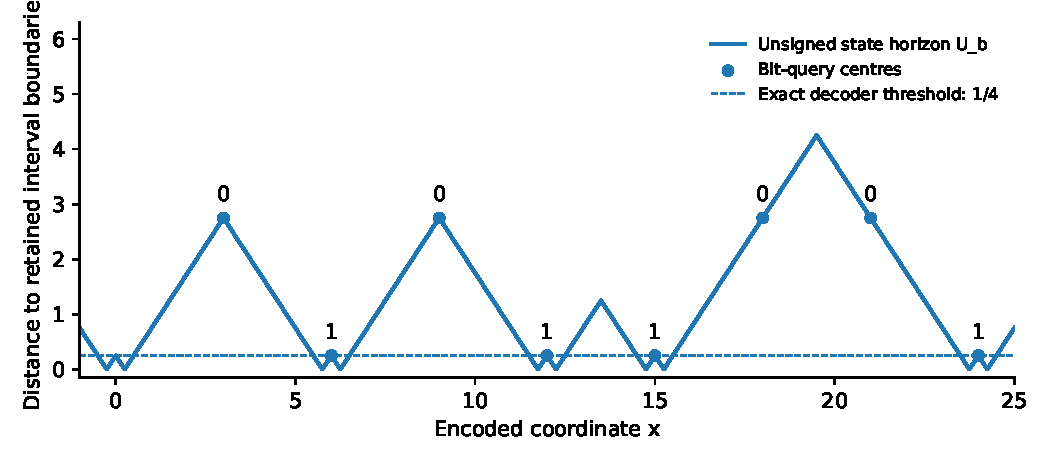
\includegraphics[width=\textwidth]{figures/unsigned_state.pdf}
\caption{The word 01011001 represented entirely by nonnegative boundary distances. Query values at active centers are $1/4$; the zero set lies on retained interval endpoints.}
\end{figure}

\subsection{The exact unsigned transition wrapper}
On the image of the complete encoding, define
\begin{equation}
F_\sigma=E_\sigma T_\sigma E_\sigma^{-1},
\qquad \Psi_{U,\sigma}=J_UF_\sigma J_U^{-1}.
\end{equation}
Then
\begin{equation}
F_\sigma E_\sigma=E_\sigma T_\sigma,
\qquad\Psi_{U,\sigma}J_U=J_UF_\sigma.
\label{eq:commutation}
\end{equation}
The executable wrapper decodes the complete unsigned state, advances the unchanged integer law, and encodes the resulting complete word. Its 64-update demonstration is checked against direct execution at every update.

For a cell index $i$ and local zero-based bit $k$, the one-based complete-word symbol is
\begin{equation}
j(i,k)=28+118i+k.
\end{equation}
The previous pulse is local bit 115, so its complete position is $j_q(i)=143+118i$. In particular, cell 7 uses symbol 969 and one-dimensional query coordinate 2907. These offsets include the 27 global control bits. They connect the source's one-bit self-feedback to an exact complete-field address.

\subsection{UU8. A lossless log-polar address lift}
The source's planar chart gives a cell center $p_i=p_{y_i x_i}$. Its 118 bits need separate addresses. V2 introduces a positive layer spacing $h$ and the following three-dimensional address map:
\begin{equation}
\Phi(j)=\begin{cases}
(0,0,(j-1)h),&1\le j\le27,\\
(p_{i,x},p_{i,y},kh),&j=28+118i+k,\quad0\le k<118.
\end{cases}
\label{eq:lift}
\end{equation}
The first branch is a dedicated control axis. A permanent anchor is placed at $(0,0,-h)$. All cell centers have positive radius, so they are distinct from the control axis. Radial indices, angular indices and layer indices each remain distinguishable. This is an explicit V2 lift of the mapping requested on S3 pages 16--18.

Let $r_0=1/32$, $q=128^{1/(R-1)}$ and
\begin{equation}
\delta_*=
\min\left\{h,\ r_0,\ 2r_0\sin(\pi/A),\ r_0(q-1)\right\}>0.
\end{equation}
Every distinct pair of address centers, including the permanent anchor, is separated by at least $\delta_*$. Different layers or control heights are separated by $h$; cell and control centers by at least $r_0$; different angular positions on the innermost row by at least the stated chord; and different rows by at least the radial gap.

Choose $a_3=\delta_*/4$. Around the anchor and every active address, place a sphere horizon of radius $a_3$. The exact Euclidean unsigned boundary field is
\begin{equation}
U_b^{(3)}(P)=\min_{c\in\{c_0\}\cup\{\Phi(j):b_j=1\}}
\left|\|P-c\|-a_3\right|.
\end{equation}
At an active query center its value is $a_3$; at an inactive one it is at least $3a_3$. The word is therefore recovered with any threshold in $[a_3,3a_3)$. This proves the injectivity of the lifted representation.

The planar projection alone does not retain the layer coordinate. Nor does the log-polar map generally preserve Euclidean distances. The 1D exact horizon keeps its own metric; the lifted 3D family is built from newly specified Euclidean sphere primitives and its stated separation radius. Its information-preserving relation to the word is the proved address-and-query map.

\begin{figure}[H]
\centering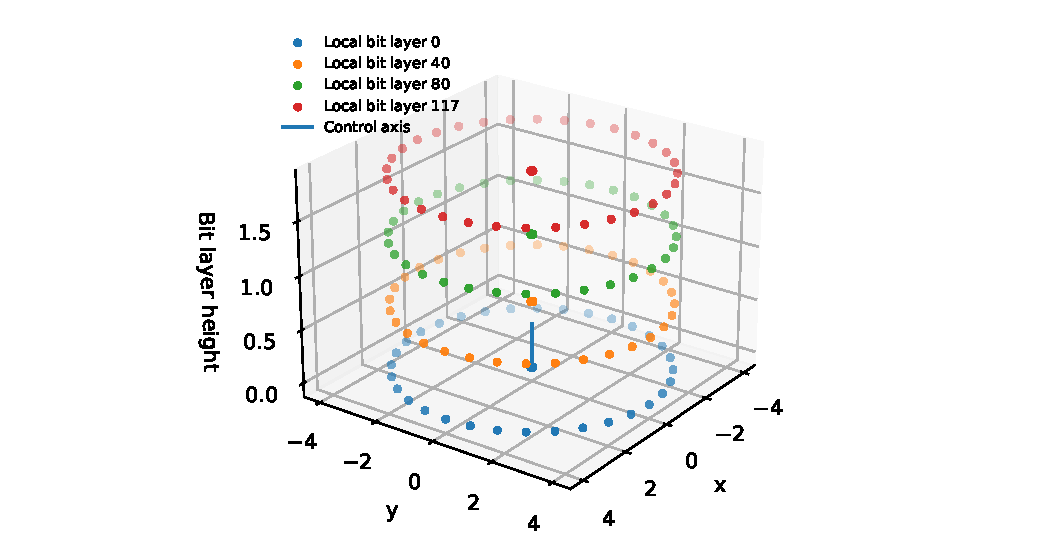
\includegraphics[width=\textwidth]{figures/logpolar_layers.pdf}
\caption{Four displayed layers from the full 118-layer address lift for the 64-cell fixture. The separate control axis preserves all 27 global bits. All 7,579 addresses are included in the archive's CSV.}
\end{figure}

\subsection{UU9. The historical state envelope is Boolean OR}
For two words of the same length, $a\lor b$ retains exactly the interval centers present in either word. The anchor is common. Thus
\begin{equation}
J_U(a\lor b)=\min\{J_U(a),J_U(b)\}.
\label{eq:or-homomorphism}
\end{equation}
For a finite state trajectory with words $b_0,\ldots,b_n$,
\begin{equation}
\min_{0\le k\le n}U_{b_k}
=J_U\left(\bigvee_{0\le k\le n}b_k\right).
\end{equation}
This gives the source's ``UU ID over the invariant orbit'' a precise operation on the C13 state family. The proof is equality of the selected center sets, followed by equality of their minimum boundary fields. \src{S3}{pp. 14--15}

The historical OR word is monotone in each bit and can change strictly at most $B$ times. This bounds the number of strict changes, not the update index at which the last change occurs. If the engine orbit has preperiod $\mu$ and period $p$, every future state already occurs among the first $\mu+p$ states, so the envelope has stabilized by their inclusion.

The envelope generally loses chronology and the designation of the current state. The same historical OR can result from different ordered histories or endpoints. V2 therefore stores \emph{current-state horizon}, \emph{historical envelope} and \emph{labelled lineage} as different fields of Equation~\eqref{eq:identity-object}. Only the complete current state is passed to the unchanged autonomous transition.

\newsec{Unified Field Theorem V2}
\label{sec:theorem}
\origin{U4: S2, §4. UF2: V2 construction from the retained engine, literal registry and UU ID definitions.}

\subsection{The retained operational closure theorem}
\begin{formal}{U4. Unified operational closure}
Fix a complete admitted seed $\sigma$, its immutable lookup bytes and the ordered integer transition $T_\sigma$. Let $\mathsf S_\sigma$ be the states satisfying the cell and control bounds and the fixed positive material total.

Then $T_\sigma$ is a uniquely defined endomorphism of $\mathsf S_\sigma$. Every finite iterate remains in this domain, conserves $M_0$ and emits uniquely determined Boolean planes. The complete encoding $E_\sigma$ is injective, with length $118N+27$ and an inverse on its image. For every cell and every finite segment,
\[
D Q_i(t)+r_i(t)=r_i(0)+K_i(t),\qquad
Q_i(t)=\sum_{n<t}q_i(n),\quad K_i(t)=\sum_{n<t}z_i(n+1).
\]
A complete capsule restores the same future transition inputs and therefore the same continuation. The operational orbit is eventually periodic.
\end{formal}
The mathematical assumptions are the stated exact arithmetic, fixed seed and completed old/new stages. The supporting proofs are retained in Section~\ref{sec:proofs}. These assumptions are the domain of the theorem and remain explicit in its unsigned representation.

\subsection{The V2 unification theorem}
Let $\mathfrak D_\sigma$ be a finite referentially closed registry binding the author record, seed, transition and all used representation maps. Define the fixed-registry realization
\begin{equation}
\mathbb S_\sigma=\{(\mathsf a_{\rm TK},\mathfrak D_\sigma,\sigma,S):S\in\mathsf S_\sigma\}.
\end{equation}
Its operative update holds the first three entries fixed and advances $S$. The unsigned representation of the state is $\mathcal J_\sigma=J_UE_\sigma$.

\begin{formal}{UF2. UU ID referential and representational unification}
Under the hypotheses of U4 and referential closure of $\mathfrak D_\sigma$:

\textbf{State closure.} The map
\[
\mathbb T_\sigma(\mathsf a_{\rm TK},\mathfrak D_\sigma,\sigma,S)
=(\mathsf a_{\rm TK},\mathfrak D_\sigma,\sigma,T_\sigma S)
\]
is a total deterministic endomorphism of the stated fixed-seed realization. Author attribution, definition records and content addresses are invariant under this operative update.

\textbf{Unsigned field equivalence.} The map $\mathcal J_\sigma$ is injective. On its image,
\[
\Psi_{U,\sigma}=\mathcal J_\sigma T_\sigma\mathcal J_\sigma^{-1},
\qquad\Psi_{U,\sigma}\mathcal J_\sigma=\mathcal J_\sigma T_\sigma.
\]
The complete unsigned field carries exactly the operative state information needed for continuation.

\textbf{Composition.} Finite UU ID composition obeys UU1--UU3. In the fixed C13 family, it commutes with Boolean OR according to UU9. Tagged composition additionally retains all declared component identities and minimizer records.

\textbf{Spatial lift.} The log-polar layered construction of UU8 is another injective representation of the complete word, with an explicit center-query inverse on its image.

\textbf{Chronotemporal extension.} Every finite supplied experience sequence satisfying the stated record, parent, timing and integrability conditions admits the lineage append, historical minimum and fixed-query integral operations defined in this volume. Their outputs are uniquely determined by those declared inputs and conventions.
\end{formal}
\begin{proof}
The constant entries of $\mathbb T_\sigma$ preserve the attribution and registry. U4 gives the total invariant-preserving update on the operative entry. C11 and UU6 make $\mathcal J_\sigma$ a composition of injections with an explicit inverse on its image. Substitution proves the conjugacy identity. UU1--UU4 prove the finite composition and tagged-record statements, while UU9 identifies the historical state union with Boolean OR. UU8 proves distinct addresses, separated sphere horizons and their decoder. The experience append rule uses only already committed parents; induction preserves its acyclic graph and previous records. Each finite historical minimum and each admitted integral is defined by its given input data, establishing the final assertion.
\end{proof}

\begin{figure}[H]\centering
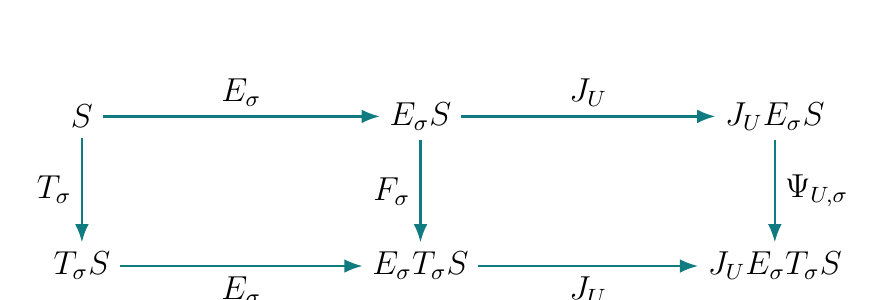
\begin{tikzpicture}[>=Latex,every node/.style={font=\large},a/.style={->,draw=teal,line width=.8pt}]
\node (s) at (0,0) {$S$};\node (b) at (4.3,0) {$E_\sigma S$};\node (u) at (8.8,0) {$J_UE_\sigma S$};
\node (ns) at (0,-1.9) {$T_\sigma S$};\node (nb) at (4.3,-1.9) {$E_\sigma T_\sigma S$};\node (nu) at (8.8,-1.9) {$J_UE_\sigma T_\sigma S$};
\draw[a] (s)--node[above]{$E_\sigma$}(b);\draw[a] (b)--node[above]{$J_U$}(u);
\draw[a] (ns)--node[below]{$E_\sigma$}(nb);\draw[a] (nb)--node[below]{$J_U$}(nu);
\draw[a] (s)--node[left]{$T_\sigma$}(ns);\draw[a] (b)--node[left]{$F_\sigma$}(nb);\draw[a] (u)--node[right]{$\Psi_{U,\sigma}$}(nu);
\end{tikzpicture}
\caption{The same current-state update in operative, binary and unsigned UU ID coordinates. Inverse maps are defined on their representation images.}
\end{figure}

\subsection{Current state, history and autonomous recurrence}
U4's finite state is the current operative word. Its augmented lineage may append a new record at every update, even when the operative word repeats. A history supplied externally is an input to the chronotemporal extension; it is not silently introduced into the autonomous $T_\sigma$. A deterministic observer of the numerical trajectory can instead define an autonomous append rule on the larger state space that explicitly contains the history.

The finite-state recurrence and the ever-appended lineage therefore apply to different state domains. The historical UU ID projection over C13 words has the separate finite stabilization result UU9. This three-way distinction formalizes the source's invariant orbit, retained identity envelope and expanding experiential lineage together.

\subsection{The source's four closure structures}
Functional closure is the typed endomorphism $T_\sigma:\mathsf S_\sigma\to\mathsf S_\sigma$. Geometric/topological organization consists of the declared support graph, quotient maps and the proved representation geometries. Parity is a specific Boolean observation of each packed word. Temporal closure is the bounded operative phase/cooldown description, together with the independently specified history operations.

The unified registry holds these structures as typed definitions. The commuting maps connect complete state and geometry. The tagged union and lineage maps connect scalar boundary evaluation to retained identity records. These are the explicit mathematical relations associated with the source's common identity vocabulary. \src{S2}{§§4 and 8}; \src{S3}{pp. 13--18}

\newsec{Supporting proof family C1--C16}
\label{sec:proofs}
\origin{Retained proof topics and equations: S2, §5, physical pp. 10--14.}

\subsection*{C1. Initialization and finite addressing}
The admitted dimensions give $N\le2^{22}$ and at most $5N$ texels. The lookup index $(gR+y)A+j$ is at most $5N-1$ and fits an unsigned 32-bit address. Angular indices are reduced modulo $A$, and radial edges are included only where their endpoints exist. Initialization gives all required registers values inside the stated domain. The explicit zero-material branch and positive memory divisor make every division defined. Every read refers to a fixed parameter, texel or completed old-state value.

\subsection*{C2. Finite generative closure}
The rewriting map is total on its alphabet, so a finite input word has one finite output word. The branch brackets inserted by the two productions are balanced. Each drawing symbol produces three drawing symbols, giving $n_g=2\cdot3^g$ from either paired axiom. The interpreter and finite generation selection give a finite baked asset. Online generation growth selects a stored level within the fixed range.

\subsection*{C3. Shared edge law and nonnegative transport}
A node has at most four neighbors and each outgoing transfer is at most one eighth of its source count. Therefore
\begin{equation}
\sum_jJ_{i\to j}\le M_i/2,
\qquad M_i-\sum_jJ_{i\to j}\ge0.
\end{equation}
Incoming transfers are nonnegative. Each directed amount is computed from the same old source count and symmetric edge law at both endpoints. It appears once negatively at its source and once positively at its destination. Summing all cells cancels every internal transfer, giving $\sum_i\widetilde M_i=\sum_iM_i$ for each species.

\subsection*{C4. Conservative reaction}
The positive reaction shifts ensure $0\le\alpha_i\le\widetilde U_i$ and $0\le\beta_i\le\widetilde V_i$. The two next species are nonnegative. Adding their updates gives
\begin{equation}
U_i'+V_i'=\widetilde U_i+\widetilde V_i.
\end{equation}
With C3 this preserves the global total $M_0$. Each individual count is consequently at most $M_0<2^{32}$, so its stored width suffices.

\subsection*{C5. Recurrence and intermediate bounds}
Clipping gives $0\le A_i\le D$. The material-ratio observation and its zero-total branch are in the same interval. Each activity or memory recurrence is a floored convex combination of values in $[0,D]$, so $v_i,z_i',m_i'\in[0,D]$.

For integer memory divisor at least one, $|h_i|\le32768$, giving $F_i\in[-65536,65535]$. The specified coefficients fit the declared sample-drive intermediate ranges. The numerator $DU_i'$ is less than $2^{48}$, and the largest declared growth product is at most $2^{38}$; the stated 64-bit intermediates contain them. The Python realization evaluates these as exact integers.

\subsection*{C6. Pulse codec and finite-segment certificate}
Since $0\le r_i<D$ and $0\le k_i\le D$, the sum satisfies $0\le r_i+k_i<2D$. The threshold selects a bit, and subtracting $Dq_i$ leaves $0\le r_i'<D$. Summing Equation~\eqref{eq:pulse} over a finite segment cancels intermediate residuals:
\begin{equation}
DQ_i(t)+r_i(t)=r_i(0)+K_i(t).
\end{equation}
Hence
\begin{equation}
Q_i(t)-K_i(t)/D=(r_i(0)-r_i(t))/D,
\qquad |Q_i(t)-K_i(t)/D|<1.
\end{equation}
A segment beginning at zero residual additionally satisfies $-1<Q_i-K_i/D\le0$. Restored segments use their actual starting residual. Adjacent certificates compose by cancelling the shared endpoint residual.

\subsection*{C7. Hysteresis and the event telescope}
For $H>0$, the two outer threshold conditions are disjoint. Each assigns a bit, and the middle branch preserves the old bit. The latch therefore remains Boolean. Since each intermediate latch occurs twice under XOR,
\begin{equation}
\bigoplus_{n<t}e_i(n)=\ell_i(0)\xor\ell_i(t).
\end{equation}
Occupancy is separately defined from the present threshold relation. UU7 preserves all these facts under the open relational lift.

\subsection*{C8. Exact packing and parity}
Distinct Boolean positions occupy distinct powers of two. Packing by their OR or sum and extracting the same position are inverse operations. The old pulse word reconstructed from flags therefore provides exactly the pulse read specified by the sampler. Word parity is the XOR of its data bits; for an error mask $e$,
\begin{equation}
\operatorname{parity}(w\xor e)=
\operatorname{parity}(w)\xor\operatorname{parity}(e).
\end{equation}
Odd-weight masks change parity and even-weight masks preserve it. The complete word and the parity observation have distinct data types and different information content.

\subsection*{C9. Bounded phase and cooldown quotient}
The older operative equations in S2's comparison read time through $ns\bmod A$ and elapsed dwell through its comparison with $d_{\rm dwell}$. Their sufficient-state projection keeps
\begin{equation}
a=ns\bmod A,\qquad
c=\min(d_{\rm dwell},n-\mathrm{lastGrowth}),
\end{equation}
and the operative cells and current generation. Modular addition preserves phase. For nonnegative elapsed time $e$,
\begin{equation}
\min(d,\min(d,e)+1)=\min(d,e+1).
\end{equation}
A growth event resets both descriptions' elapsed dwell to zero. Observer totals not read by the operative recurrence can remain external. The projected and bounded-state transitions consequently commute on the admitted comparison domain. \src{S2}{C9}

\subsection*{C10. Boolean arithmetic refinement}
For bits $a,b,c$, the full adder is
\begin{equation}
s=a\xor b\xor c,
\qquad c'=(a\land b)\lor((a\xor b)\land c).
\end{equation}
Its eight input cases give $a+b+c=s+2c'$. Induction over digit positions proves ripple addition. Complement-plus-one gives modular negation; adding it gives subtraction. Borrow propagation gives unsigned comparison, fixed shifts route digits, and selected shifted additions give multiplication.

For restoring division by $d>0$, maintain $0\le R<d$ while consuming one numerator bit. The trial $2R+a_i$ is less than $2d$. Subtract $d$ exactly when the trial is at least $d$, emit that quotient bit and retain the remainder. A $w+1$-bit temporary preserves the trial carry. Induction gives the quotient and remainder. Signed memory division applies this to magnitudes and restores the sign, yielding truncation toward zero. The width bounds in C5 ensure these primitives realize the intended integer values.

\subsection*{C11. Complete state encoding and restart}
Each cell requires $32+32+17+17+16+4=118$ bits; controls require $11+3+13=27$. Sequential insertion and extraction with the same field order are inverse operations. The unused final padding bits are fixed to zero.

The complete restart capsule carries the immutable seed, material descriptor and encoded operative state. Reconstructing flags reconstructs the old packed output planes. Every causal input to the next transition is thus recovered. Encode/decode is the identity on accepted states, and induction over later transitions proves exact continuation after a pause.

\subsection*{C12. Autonomous closure and eventual periodicity}
C1 makes the transition defined. C3--C7 preserve the cell domain and material total. Modular phase, bounded generation and saturating cooldown preserve control. Hence $T_\sigma(\mathsf S_\sigma)\subseteq\mathsf S_\sigma$ and every finite iterate exists uniquely.

The injection into a $B$-bit word gives $|\mathsf S_\sigma|\le2^B$. A trajectory must eventually repeat a state, after which determinism repeats its future. There are $\mu\ge0$ and $p\ge1$ with
\begin{equation}
S_{n+p}=S_n\quad(n\ge\mu),
\qquad \mu+p\le|\mathsf S_\sigma|\le2^{118N+27}.
\end{equation}
This is eventual periodicity of the operative state. The separate historical minimum has the stabilization property of UU9, while an appended lineage retains its explicitly growing record domain.

\subsection*{C13. Exact signed-distance state representation}
For Equation~\eqref{eq:c13}, define
\begin{equation}
d_b(x)=\begin{cases}
-\dist(x,\mathbb R\setminus\Omega_b),&x\in\Omega_b,\\
\dist(x,\Omega_b),&x\notin\Omega_b.
\end{cases}
\end{equation}
At an active center $3j$ the value is $-1/4$, and at an inactive center it is positive. Therefore $b_j=\ind\{d_b(3j)<0\}$, proving the original injection. Its conjugate transition is defined by encoding, advancing and decoding on the image. V2's UU6 gives the corresponding complete nonnegative horizon and a different, explicitly proved decoder.

\subsection*{C14. Exact reduced-description criterion}
For a proposed reduction $e:\mathsf S\to Y$ and observation $h:\mathsf S\to O$, reduced functions $\overline T$ and $\overline h$ with $eT=\overline Te$ and $h=\overline he$ exist precisely when
\begin{equation}
e(s)=e(t)\Longrightarrow
\big(e(Ts)=e(Tt)\ \text{and}\ h(s)=h(t)\big).
\end{equation}
Necessity follows by substitution. For sufficiency, define the reduced functions using one representative of each fibre; the stated condition makes the choice immaterial.

The previous pulse alone is not a sufficient reduction of the admitted state. Keep every value except one residual fixed, with old $z=D/2$. The next activity $k$ is independent of that residual and lies in $[3D/8,5D/8]$. Residuals zero and $D-k$ have the same old pulse observation but produce next pulses zero and one. The full residual remains operative information.

\subsection*{C15. Causal use of prior output}
The source's constructive experiment changes one designated read of a previous output bit while holding the incoming state and all earlier execution fixed. The bit enters the next lookup address and direct drive, so a difference can propagate to later state and output. S2 records this on its verification XY seed. \src{S2}{C15}

V2 separately instantiates the experiment on its declared integer-chart fixture: only cell 7's read at zero-based tick 3 is inverted. The first operative-state difference is at tick 3 and the first pulse-plane difference at tick 9. The source's own verification XY example instead records the first output difference at tick 7. Both records retain their own seed and experiment identity.

\subsection*{C16. Staged backend refinement}
An implementation realizes the same transition when it uses identical seed data, arithmetic, indices and completed old/new stages. Equal incoming states yield equal sample arrays. Equal samples and old neighbors yield equal transported material. The ordered local reaction, recurrence, codec and hinge give equal next cells; their completed flags give equal words and pulse totals; and bounded control yields equal next controls. Induction proves trajectory equality under those stage contracts.

For a parallel implementation, every next cell and packed word has one owner, neighbor reads use completed old state, and padding lanes contribute false during packed-word operations. The V2 delivered implementation executes the Python integer and unsigned-field paths. The digit-array arithmetic module supplies the concrete Boolean constructions tested for C10; it is not labelled a separately executed full-engine backend.

\newsec{Retained geometry, topology and Dutch number calculus}
\label{sec:retained}
\origin{Retained definitions and examples: S1, §§4--8.}

\subsection{Geometric definitions and local charts}
A parametric family is $\gamma:U\to\mathbb R^m$ with a declared parameter domain, regularity and frame rule. A retained implicit field declares its scalar codomain and membership convention. The inherited CSG expressions
\begin{equation}
f_{A\cup B}=\min(f_A,f_B),\qquad
f_{A\cap B}=\max(f_A,f_B),\qquad
f_{A\setminus B}=\max(f_A,-f_B)
\end{equation}
are its signed membership compositions. The open UU ID composition in V2 has its separately declared boundary-retention semantics from Section~\ref{sec:uuid}. \src{S1}{\S4.1}; \src{S3}{pp. 1--3}

For $b\ge2$, exact radix digit thresholds occur at $b^k$. The digit count is one at zero and $\lfloor\log_b n\rfloor+1$ for positive $n$. The archive's integer routine determines the digits by repeated division. The thresholds can address shells $[b^k,b^{k+1})$.

For $r>0$, a local log-polar chart is $\rho=\ln(r/r_0)$ and $\theta=\operatorname{atan2}(y,x)$. The origin has an explicit core flag. In the V2 3D lift, the control axis belongs to a separate address branch rather than being passed through the singular planar log-polar formula. \src{S1}{\S4.2}

\subsection{Pulse polygons and Pascal occupancy}
A declared positive pulse count $m$, radius $r>0$ and phase $\phi$ define ordered vertices
\begin{equation}
p_j=r\big(\cos(\phi+2\pi j/m),\sin(\phi+2\pi j/m)\big),
\qquad0\le j<m.
\end{equation}
One pulse yields a point, two a segment, and higher counts a regular polygon. Pulse identity and source positions are stored as metadata. The Pascal mask is
\begin{equation}
P(n,k)=\binom nk\bmod2
=\ind\{k\mathbin{\&}(\mathord{\sim}n)=0\},\qquad0\le k\le n.
\end{equation}
Over the two-element field, $(1+x)^{2^j}=1+x^{2^j}$. Factoring by the active bits of $n$ shows that an odd coefficient occurs exactly when the active bits of $k$ are a subset of those of $n$. In particular, every coefficient in row $2^q-1$ is odd. \src{S1}{\S2.2; P36-03}

\subsection{Topology and hinge composition}
A gluing record names entry/exit ports, coordinate transport, orientation transport, optional sheet change and lineage update. The M\"obius-style map is
\begin{equation}
(0,y,o)\sim(w,h-y,-o).
\end{equation}
Applying the transverse reversal twice restores coordinate and orientation. A declared sheet bit may be toggled with each crossing. Compatibility can separately require equal sheet, phase or branch before a coupling is admitted. \src{S1}{\S5.1}

For a fixed pivot $p$, the continuous hinge is
\begin{equation}
x'(t)=p+R(\theta(t))(x-p),\qquad
\dot x'(t)=\dot\theta(t)JR(\theta(t))(x-p),
\quad J=\begin{pmatrix}0&-1\\1&0\end{pmatrix}.
\end{equation}
A parity hinge chooses a map. A connector hinge inserts structural incidence with its declared magnitude. The stored chain $M_n\circ\cdots\circ M_1$ is generally non-commutative. These are the retained map families used by S3's extension to temporal connectors. \src{S1}{§§5.2--5.3}; \src{S3}{p. 10}

\subsection{Dutch place order and spoken identity}
For $n=10t+u$, with $2\le t\le9$ and $1\le u\le9$, the place and spoken charts are
\begin{equation}
P(n)=(10t,u),\qquad S_{\rm nl}(n)=(u,\mathrm{en},10t).
\end{equation}
The connector hinge is $H_{\rm en}(10t,u)=(u,\mathrm{en},10t)$, with $\val(\mathrm{en})=0$. Therefore
\begin{equation}
\val(P(n))=\val(S_{\rm nl}(n))=n.
\end{equation}
The connector changes graph structure and spoken order while preserving numerical value. For 13--19, the unit root precedes the suffix \emph{tien}; eleven and twelve remain separate irregular lexemes. \src{S1}{\S6.2}

A profile segment sequence $\Sigma_{\rm nl}(n)=(s_1,\ldots,s_m)$ gives one pulse per segment. Independently, $A_2(n)=\{k:\operatorname{bit}_k(n)=1\}$ gives the active binary positions. The comparison is
\begin{equation}
M(n)=\ind\{m=|A_2(n)|\}.
\end{equation}
This Boolean comparison is retained as a feature observation. Both the numerical value and the source metadata remain in the literal instance. \src{S1}{\S6.3}

\subsection{Worked records: 19 and 23}
For 19,
\begin{equation}
19=16+2+1=(10011)_2,\qquad A_2(19)=\{0,1,4\}.
\end{equation}
The edition profile gives \emph{ne / gen / tien}, so the pulse count and binary Hamming weight are both 3. The unit-radius three-pulse embedding is
\begin{equation}
(1,0),\quad(-1/2,\sqrt3/2),\quad(-1/2,-\sqrt3/2),
\end{equation}
with area $3\sqrt3/4$. Source bit positions 0, 1 and 4 remain attached to the record.

For 23, the place chart $(20,3)$ maps to \emph{drie--en--twintig}. The profile segments are \emph{drie / en / twin / tig}. Its active binary positions are $\{0,1,2,4\}$, and the four-pulse embedding is a square. These examples preserve the structural connector used in S3's temporal-hinge interpretation. \src{S1}{§§6.4 and 9.3}

The complete V2 profile \texttt{nl-TKUFT-0-99-v2} is generated from explicit unit, teen and tens dictionaries and the two connector rules. Its full matching set is
\begin{equation*}
\begin{split}
\{&1,2,4,8,9,18,19,20,23,40,43,45,46,47,51,53,54,\\
&58,59,70,80,83,85,86,87,91,93,94\}.
\end{split}
\end{equation*}
It contains 28 values, matching the total printed in S1. All 100 rows, their explicit segmentation and their count-comparison fields are included as CSV and JSON. The full dictionary table is an edition profile following the source's printed morphology and examples.

\newsec{Executable V2 and recorded verification}
\label{sec:verification}
\origin{All results in this section are generated by the delivered V2 code and explicit examples.}

\subsection{The integer-chart fixture}
The numerical fixture is \texttt{TKUFT-integer-chart-v2}, with $A=32$, $R=2$, $G=2$ and $N=64$. Its 128 immutable lookup texels are generated from
\begin{equation}
d_{gyx}=128\left|((x+8)\bmod32)-16\right|+96y-1152-256g.
\end{equation}
The drive is $c_{gyx}=\clip_{[0,65535]}(32768-16d_{gyx})$, and the packed texel uses the same two-code layout as the retained engine. This is a direct integer-code fixture constructed for the edition.

For initial active cells with $d_{0,y_i,x_i}\le0$,
\begin{equation}
U_i=256+17((11i+3)\bmod13),\qquad
V_i=128+7((5i+1)\bmod11).
\end{equation}
Inactive cells start with both counts zero. All cells start at $z=m=D/2$, $r=0$ and flags zero; control starts at $(0,0,0)$. The resulting material total is 18,677. The coefficients are the defaults stated in Section~\ref{sec:engine}, with feedback enabled.

\subsection{Direct and unsigned-field execution}
\begin{center}
\begin{tabularx}{\textwidth}{@{}Xr@{}}
\toprule\textbf{Recorded quantity} & \textbf{Result}\\\midrule
Executed unit-test methods & 126 passed\\
Content-addressed definition records & 34 verified\\
Retained operators / UU ID mechanisms / pattern recipes & 36 / 16 / 20\\
Dutch profile entries / count matches & 100 / 28\\
Direct engine updates & 64\\
Matched unsigned-field conjugate updates & 64\\
Initial and final material total & 18,677\\
Emitted pulse symbols equal to one & 2,258\\
Pulses in the final update & 38\\
Complete operative word & 7,579 bits\\
Byte-padded operative payload & 948 bytes\\
Local finite-segment certificates & 64 of 64 passed\\
Restored and uninterrupted final states & Equal\\
Historical OR-envelope active positions & 4,262\\
Strict envelope changes during the run & 57\\
\bottomrule
\end{tabularx}
\end{center}

The final operative-payload SHA-256 is
\begin{center}\small\ttfamily
77f7cdbf7ce5f76029d5d6c27900187b7edb\\
df12f0ecbbe664db21f3fd6b9d8b
\end{center}
Each field-wrapper update decodes all 7,579 bits, reconstructs the state, applies the integer law and builds the next exact unsigned horizon. Equality is checked against direct execution at every update. The historical envelope includes the initial word and all 64 subsequent words. It is stored separately and is not used as the current-state restart payload.

\subsection{Causal feedback record}
The one-read experiment inverts the prior-output read at cell 7, tick 3, exactly once. The first operative difference is at tick 3 and the first output-plane difference at tick 9. The first 40 cell-7 pulse symbols are
\begin{lstlisting}
Baseline:     0101011010110100101010101010110110110111
Intervention: 0101011011010101001010101010110110111011
\end{lstlisting}
\begin{figure}[H]\centering

\includegraphics[width=\textwidth]{figures/feedback.pdf}
\caption{The edition's recorded one-read intervention. This figure and its CSV are specific to the stated integer-chart seed.}
\end{figure}
The matched feedback-mode-zero seed emits 2,235 ones through the same 64-update interval and preserves the same material total. This is a separate mode comparison, not the one-read intervention.

\subsection{UU ID, experience and spatial examples}
The elementary UU ID example uses one-dimensional sphere horizons $|x|=1$ and $|x-3|=1$. At $x=1.5$, both normalized deviations are 0.5. The scalar UU ID is 0.5 and the tagged result contains both minimizing IDs, \texttt{A} and \texttt{B}.

The absorption example is an explicitly synthetic fixed-query profile: four unit-duration segments with comparison values $(2,4,1,3)$ and $\lambda=0.5$. Its integral is approximately 4.347292234638. The retention mass is approximately 1.729329433527. Dividing gives the optional normalized observation 2.513860083774. The normalization is recorded as a derived statistic; the integral itself remains the source-defined observable.

The synthetic boundary history has centers $0,0.25,0.5$, each with threshold 1, committed at times 0, 1 and 2. Consecutive center distances are 0.25, so the declared $\varepsilon=0.25$ path condition holds. Its historical horizon at query 1.5 is zero after inclusion of the final component. A separate four-node split--merge example records two parents at its merge and verifies their content addresses.

The full spatial address CSV has 7,579 rows. For the chosen layer spacing $h=1/64$, the separation and sphere radius are
\begin{equation}
\delta_*\approx0.006126071270598,
\qquad a_3\approx0.001531517817649.
\end{equation}
Each row names its global symbol, control or cell role, local cell bit, three-dimensional coordinate and current bit value.

\subsection{Test scope and data verification}
The test suite contains 63 retained-core tests and 63 UU ID/identity/wrapper tests. It checks canonical records, dependency resolution, radix and Pascal calculations, hinges, the Dutch profile, exact integer dynamics, state/capsule reconstruction, the UU ID algebra, tagged minimizers, all 256 eight-bit unsigned encodings, integral recurrence, lineage integrity, the relational hinge and the spatial address lift.

The arithmetic tests include all 65,536 pairs of 8-bit addition inputs, all pairs of 5-bit inputs for subtraction/comparison and multiplication, all 5-bit numerator/nonzero-divisor pairs, and deterministic 64-bit division cases. The numerical tests include 512 updates with material, pulse-certificate and latch-event checks; a gather/scatter transport comparison; and a 23-plus-41-update restart split. The full demonstration separately checks 64 direct/unsigned updates and a half-run restart split.

Both JSON Schema documents are checked, and the example substrate validates against the corpus schema. Verification records distinguish unit tests, schema validation, regenerated data and deterministic replay. File integrity is checked by the delivered SHA-256 manifest.

\subsection{Reproduction and capsule use}
From the extracted archive root:
\begin{lstlisting}
python tools/verify.py
python examples/run_demo.py --out demo_run --steps 64
\end{lstlisting}
The runtime and test suite use the Python standard library. The verifier checks the manifest, definitions, complete profile, tests and freshly generated demonstration. Its optional \texttt{--schema} flag uses the separately listed JSON Schema validation dependency.

The edition's \texttt{TKUFT2} capsule contains the complete numerical seed, code array, material total, declared bit length, encoded state and a digest over the canonical payload. The wrapper-specific \texttt{state\_horizon.json} additionally exposes the complete bit word and its horizon parameters. These edition formats preserve the source's operative field order while using their own explicitly named envelopes.

\begin{lstlisting}
from pathlib import Path
import sys
sys.path.insert(0, "src")
from tkuft.codec import decode_capsule, encode_capsule
from tkuft.engine import tick

seed, state = decode_capsule(
    Path("verification/demo/final.tku").read_bytes())
for _ in range(64):
    state, summary = tick(seed, state)
Path("continued.tku").write_bytes(encode_capsule(seed, state))
\end{lstlisting}
The manuscript and figure generators are included. Rebuilding the PDF uses the stated LaTeX packages; regenerating the calculated plots uses matplotlib. Existing generated figures and tables are already included in the archive.

\clearpage
\subsection{V2 synthesis}
The source's central operator is preserved as an exact equation:
\begin{equation}
\uu\big((d_1,T_1),(d_2,T_2)\big)=
\min\{|d_1-T_1|,|d_2-T_2|\}.
\end{equation}
V2 places that equation inside a complete identity architecture: raw relations retain comparison state; tagged records retain component identity; the integral retains temporally weighted experience; the historical minimum retains a boundary envelope; lineage retains ancestry and order; and the full unsigned current-state field retains the information required for exact continuation.

The three principal connections are
\begin{equation}
\Psi_{U,\sigma}J_UE_\sigma=J_UE_\sigma T_\sigma,
\qquad J_U(a\lor b)=\min(J_Ua,J_Ub),
\end{equation}
\begin{equation}
\mathcal I(P,t+s)=e^{-\lambda s}\mathcal I(P,t)
+\int_t^{t+s}\mathcal D(P,E(\tau))e^{-\lambda(t+s-\tau)}\,\dd\tau.
\end{equation}
They connect the source's field identity, complete state, historical union and chronotemporal absorption through declared maps rather than through an unstated equivalence of labels. The author record, mathematical definitions and executable constructions are collected together as \emph{Tom Klootwijk --- Unified Field Theory V2}.

\appendix
\newsec{UU ID mechanism catalogue}
\label{app:uu}
\origin{Sixteen V2 mechanisms. Source locations and construction status are included in the companion CSV and JSON.}
The mechanisms below organize the new source around its native terminology. Source-defined equations, distinct source conventions and V2 implementation constructions have separate provenance fields.
{\small\begin{longtable}{@{}p{.10\textwidth}p{.31\textwidth}p{.54\textwidth}@{}}
\toprule\textbf{ID} & \textbf{Mechanism} & \textbf{Definition}\\\midrule\endfirsthead
\toprule\textbf{ID} & \textbf{Mechanism} & \textbf{Definition}\\\midrule\endhead
\midrule\multicolumn{3}{r}{\small Continued on the next page}\\\endfoot\bottomrule\endlastfoot
UU2-01 & Open threshold relation & d compared with T gives <, = or >\\[5pt]
UU2-02 & Agnostic Boundary Horizon & delta(x)=abs(d(x)-T)\\[5pt]
UU2-03 & UU ID Double Set Operator & min(abs(d1-T1),abs(d2-T2))\\[5pt]
UU2-04 & Tagged identity disjunction & Retain component records, minimum value and all exact minimizer IDs\\[5pt]
UU2-05 & Point-Source / Genesis Horizon & abs(norm(P-P\_source)-T\_source)\\[5pt]
UU2-06 & Source-centred one-bit convention & 0 at source, 1 away from source\\[5pt]
UU2-07 & Horizon-centred one-bit convention & 0 on threshold horizon, 1 away from horizon\\[5pt]
UU2-08 & Chronotemporal absorbing field & Integral of D(P,E(tau)) times exp(-lambda*(t-tau))\\[5pt]
UU2-09 & Historical UU ID envelope & Minimum of historical absolute threshold deviations\\[5pt]
UU2-10 & Content-addressed experience lineage & Append records with prior parents and their content addresses\\[5pt]
UU2-11 & Successive-state continuity path & Every declared successive-state distance is at most epsilon\\[5pt]
UU2-12 & Unsigned complete-state horizon & UU ID over the permanent anchor and active C13 interval boundaries\\[5pt]
UU2-13 & Unsigned state decoder & Read each bit at x=3j with a threshold in [1/4,11/4)\\[5pt]
UU2-14 & Relational engine hinge & Use F+65536 relative to 65536 and the unchanged hysteresis margins\\[5pt]
UU2-15 & Layered log-polar address lift & Keep control addresses and all 118 bit layers in a separate 3D sphere-horizon map\\[5pt]
UU2-16 & UU ID conjugate transition & Encode, decode and evolve the complete current-state horizon\\[5pt]
\end{longtable}
}

\newsec{The retained 36-operator catalogue}
\label{app:operators}
\origin{S1, Appendix A, physical pp. 18--19. Original mechanism IDs and names are retained.}
The table records the technical contracts inherited by V2. UU ID mechanisms have their own namespace and do not silently change the original IDs.
{\small\begin{longtable}{@{}p{.10\textwidth}p{.28\textwidth}p{.57\textwidth}@{}}
\toprule\textbf{ID} & \textbf{Mechanism} & \textbf{Contract}\\\midrule\endfirsthead
\toprule\textbf{ID} & \textbf{Mechanism} & \textbf{Contract}\\\midrule\endhead
\midrule\multicolumn{3}{r}{\small Continued on the next page}\\\endfoot\bottomrule\endlastfoot
K36-01 & Literal definition node & Typed definition record containing operator or object semantics.\\[5pt]
K36-02 & Content-addressed definition & Canonical JSON, excluding the content-hash field, determines the SHA-256 address.\\[5pt]
K36-03 & Explicit dependency edge & Every composed definition names its dependencies by ID.\\[5pt]
K36-04 & Versioned namespace & IDs, schema versions and profile versions distinguish definitions and semantics.\\[5pt]
K36-05 & Definition-instance separation & An instance references a definition and carries literal parameters and state.\\[5pt]
K36-06 & Acyclic resolution rule & A finite dependency graph admits a deterministic topological order.\\[5pt]
K36-07 & Typed implicit-field sign & The inherited implicit-field record declares its signed membership convention.\\[5pt]
K36-08 & Exact-SDF capability flag & Exact signed-distance status is declared for the applicable field and metric.\\[5pt]
K36-09 & Parametric curve and sweep & A curve, parameter domain, regularity class and transport rule define a family.\\[5pt]
K36-10 & Pulse polygon embedding & A positive pulse count maps to a point, segment or regular polygon.\\[5pt]
K36-11 & Radix shell chart & Powers of the radix give digit thresholds and addresses for declared nested shells.\\[5pt]
K36-12 & Log-polar core chart & The chart carries logarithmic radius, angle and an explicit singular-core flag.\\[5pt]
K36-13 & Explicit quotient/gluing map & Ports carry coordinate, orientation and optional sheet transport.\\[5pt]
K36-14 & Sheet-aware co-location & Coordinates, sheet, phase, orientation, branch and coupling policy are separate state.\\[5pt]
K36-15 & Orientation transport & Orientation follows the declared maps and transitions.\\[5pt]
K36-16 & Port and branch routing & An admitted event chooses an output port from an explicit finite routing table.\\[5pt]
K36-17 & Split-merge lineage & A split names children; a merge records all parents and their addresses.\\[5pt]
K36-18 & Guarded topology change & A topology-class change is committed through its declared transition rule.\\[5pt]
K36-19 & Generic hinge tuple & A hinge contains pivot, state, selected map, guard and invariants.\\[5pt]
K36-20 & Continuous planar hinge & A pivoted rotation defines position and differentiated velocity.\\[5pt]
K36-21 & Discrete parity hinge & A Boolean state selects one of two maps or routes.\\[5pt]
K36-22 & Connector hinge & A graph connector carries incidence and its declared numerical contribution.\\[5pt]
K36-23 & Non-commutative hinge chain & The stored order of composition is part of the hinge definition.\\[5pt]
K36-24 & Invariant subspace contract & Fixed points, axes and preserved quantities are stated in the hinge contract.\\[5pt]
K36-25 & Bounded Dutch number profile & A versioned 0--99 lexicon records spelling, segments, morphemes and hinges.\\[5pt]
K36-26 & Syllable-pulse operator & Each segment in the declared profile emits one pulse.\\[5pt]
K36-27 & Teen suffix hinge & For 13--19, the unit root precedes the suffix tien in the spoken chart.\\[5pt]
K36-28 & En connector hinge & Non-multiple tens use the order unit, en, tens.\\[5pt]
K36-29 & Spoken-place permutation & An explicit map permutes semantic components and inserts the connector.\\[5pt]
K36-30 & Feature-count comparison & A Boolean test compares pronunciation-profile pulses and binary Hamming weight.\\[5pt]
K36-31 & Phase-ordered evaluator & The ten phases run from parse and normalization to transition and lineage.\\[5pt]
K36-32 & Support-compatibility-guard discipline & Support is evaluated before compatibility and relation-guard solving.\\[5pt]
K36-33 & Deterministic trace & Each executed step records definition ID, operator kind and typed output.\\[5pt]
K36-34 & Evidence disposition & The provenance record identifies the source or formal construction of each mechanism.\\[5pt]
K36-35 & Unknown-reference and cycle rejection & Loading checks unique IDs, resolved references, verified hashes and an acyclic graph.\\[5pt]
K36-36 & Package verification contract & Schemas, tests, source hashes, file digests and reproducible examples accompany the corpus.\\[5pt]
\end{longtable}
}

\newsec{The retained 20-pattern library}
\label{app:patterns}
\origin{S1, §8, physical pp. 13--14.}
The patterns remain reusable typed recipes. V2's temporal connector and unsigned-state constructions cite the relevant inherited structures through explicit dependencies.
{\small\begin{longtable}{@{}p{.10\textwidth}p{.30\textwidth}p{.55\textwidth}@{}}
\toprule\textbf{ID} & \textbf{Pattern} & \textbf{Pipeline}\\\midrule\endfirsthead
\toprule\textbf{ID} & \textbf{Pattern} & \textbf{Pipeline}\\\midrule\endhead
\midrule\multicolumn{3}{r}{\small Continued on the next page}\\\endfoot\bottomrule\endlastfoot
P36-01 & Radix threshold ladder & integer $\to$ radix thresholds $\to$ shell indices\\[5pt]
P36-02 & Active-bit pulse simplex & integer $\to$ active positions $\to$ pulse vertices\\[5pt]
P36-03 & Pascal parity mask & (n,k) $\to$ binomial coefficient modulo two\\[5pt]
P36-04 & Dutch teen suffix hinge & 13--19 $\to$ unit-root and tien\\[5pt]
P36-05 & Dutch en-order hinge & non-multiple tens $\to$ unit, en, tens\\[5pt]
P36-06 & Cut-open boundary graph & closed edge $\to$ explicit pair of cut ports\\[5pt]
P36-07 & Loop-to-leg morph & closed arc $\to$ interpolated segment and topology record\\[5pt]
P36-08 & Split-oval antisymmetry & one loop $\to$ two oppositely displaced branches\\[5pt]
P36-09 & Overlap-lens domain & two regions $\to$ explicitly typed overlap domain\\[5pt]
P36-10 & SDF-zero event & field along trajectory $\to$ root $\to$ transition\\[5pt]
P36-11 & Cone support gate & position, axis, radius and angle $\to$ local support\\[5pt]
P36-12 & Nested-shell relevance & radius $\to$ local shell interval\\[5pt]
P36-13 & Mobius orientation wrap & boundary crossing $\to$ coordinate wrap and orientation reversal\\[5pt]
P36-14 & Klein sheet wrap & boundary crossing $\to$ wrap, orientation and sheet update\\[5pt]
P36-15 & Hourglass route table & guard, sector and parity $\to$ branch\\[5pt]
P36-16 & Log-polar bitmask & point $\to$ core flag, log radius, angle and admission bit\\[5pt]
P36-17 & Golden-angle schedule & sample index $\to$ declared angular sequence\\[5pt]
P36-18 & Bounded grammar recursion & seed and productions $\to$ finite budgeted expansion\\[5pt]
P36-19 & Event-latched field morph & continuous blend and discrete topology state $\to$ guarded commit\\[5pt]
P36-20 & Content-addressed definition graph & literal records $\to$ hashes $\to$ dependency DAG\\[5pt]
\end{longtable}
}

\newsec{Source variants and explicit V2 bindings}
\label{app:variants}
\origin{This register preserves distinct source formulations and names the executable choices made in V2.}

\subsection*{V01. Normalize first; compose second}
\textbf{Source:} S3 pp. 1--3 and 9. The central operator acts on raw values and thresholds through two absolute differences. \textbf{V2 binding:} each component is normalized once as $\delta=|d-T|$; finite composition then uses the minimum of these normalized horizon fields. Original parameters remain in the component records.

\subsection*{V02. The incomplete table row}
\textbf{Source:} S3 p. 3. The geometric-behavior table prints two complete predicates and an incomplete third row. \textbf{V2 binding:} the two complete predicates are transcribed as the source's named observations. No additional equation is reconstructed from the incomplete row.

\subsection*{V03. Weighted integral and minimum shader}
\textbf{Source:} S3 pp. 4--6. The main formula integrates retained experience with $e^{-\lambda(t-\tau)}$. The shader instead folds absolute boundary deviations with \texttt{min} and does not use $\lambda$. \textbf{V2 binding:} both are retained as separate observables, $\mathcal I$ and $\mathcal H$. The fixed-query piecewise-constant recurrence is a labelled V2 derivation of the integral.

\subsection*{V04. Source zero and horizon zero}
\textbf{Source:} S3 pp. 10--12. The prose places the zero bit at the source; the JSON places it at the equality $d=T$. \textbf{V2 binding:} \texttt{source\_bit} and \texttt{horizon\_bit} are separate functions. The executable horizon convention follows the JSON. Neither convention is silently substituted for the other.

\subsection*{V05. Component membership and whole-field decoding}
\textbf{Source:} S3 pp. 13 and 17--18; S2 C13. The local inequality $|x-3j|\le1/4$ describes an interval, and the outer loop selects active components. The local shader's \texttt{bit\_active} parameter is not used in its body; activity is checked by the surrounding loop. \textbf{V2 binding:} retain the active selection and permanent anchor, then decode the whole field through the proved center-query threshold of UU6.

\subsection*{V06. Two different 118-bit mappings}
\textbf{Source:} S3 p. 16 gives potential/occupancy/latch/trajectory labels; S2 pp. 5, 12 and 15 give the complete $U,V,z,m,r,f$ layout and global controls. \textbf{V2 binding:} the S3 labels are preserved in \texttt{source\_mapping\_view.json}. The executable word uses C11. S3 supplies no lossless conversion replacing the C11 material, memory and residual fields with that alternative view, so none is assumed.

\subsection*{V07. Finite shader sentinel and the empty minimum}
\textbf{Source:} S3 pp. 6 and 17. The accumulator is initialized to \texttt{1e6}. \textbf{V2 binding:} the mathematical empty-family value is $+\infty$. The JSON API uses an explicit empty status and null value. The permanent anchor makes complete-state horizon evaluation finite and defined at every finite query.

\subsection*{V08. Zero-based loop and one-based symbols}
\textbf{Source:} S3 pp. 16--18 uses a zero-based loop, whereas the C13 word labels are one-based. \textbf{V2 binding:} complete serialized zero-based position $k$ corresponds to symbol $j=k+1$ and center $3j$. Center zero is reserved for the permanent anchor.

\subsection*{V09. Planar chart and complete bit placement}
\textbf{Source:} S3 pp. 16--18 gives the planar log-polar equations but no complete injective placement of every local bit and global control. \textbf{V2 binding:} UU8 adds the bit-layer coordinate, dedicated control axis, permanent anchor and separation radius. The 3D field has its own Euclidean sphere metric; the planar chart is not assumed to be distance-preserving.

\subsection*{V10. Invariant orbit and expanding history}
\textbf{Source:} S3 pp. 9--10 and 14 combines ever-expanding experience with the finite state domain of S2 C12. \textbf{V2 binding:} current operative state, historical UU ID projection and append-only lineage have distinct state types. The operative trajectory is eventually periodic; the C13 historical envelope stabilizes by UU9; a newly appended lineage record remains a separate object.

\subsection*{V11. Ontology and mathematical statements}
\textbf{Source:} S3 pp. 10--15 describes the 1-bit God, Monotheistic Union, soul identity and space-as-data. \textbf{V2 binding:} these are retained as the author's named identity postulates. Theorems U4, UF2 and UU1--UU9 state the formal operations and hypotheses through which the specified representations, compositions and histories are established.

\subsection*{V12. Scalar boundary union and retained identity}
\textbf{Source:} S3 pp. 3, 9 and 11 describes preserved boundary identities and an unbroken union. \textbf{V2 binding:} the scalar minimum preserves the union of component zero sets. The tagged record preserves component labels, parameters and witnesses. A connected geometric neighborhood has the explicit overlap condition stated in Section~\ref{sec:genesis}; an identity history has its declared parent-path condition.

\newsec{Notation and source correspondence}
\label{app:notation}
\begin{longtable}{@{}p{.22\textwidth}p{.72\textwidth}@{}}
\toprule\textbf{Symbol} & \textbf{Meaning}\\\midrule\endfirsthead
\toprule\textbf{Symbol} & \textbf{Meaning}\\\midrule\endhead
\bottomrule\endlastfoot
$\mathsf a_{\rm TK}$ & The literal author record: Tom Klootwijk, NL200678942, 10-07-1990.\\[5pt]
$\mathfrak D$ & Registry of typed, content-addressed definition records.\\[5pt]
$d_\alpha,T_\alpha$ & Raw component field and its explicit threshold.\\[5pt]
$\delta_\alpha$ & Nonnegative absolute threshold deviation $|d_\alpha-T_\alpha|$.\\[5pt]
$H_\alpha$ & Zero set of the corresponding component horizon.\\[5pt]
$\uu,\dcup,U_A$ & Source Double Set Operator, normalized horizon composition and finite-family minimum.\\[5pt]
$\widehat U_A$ & Tagged evaluation retaining the scalar value, components, witnesses and raw relation records.\\[5pt]
$G,P_{\rm Source}$ & Genesis Horizon and its declared source coordinate.\\[5pt]
$b_{\rm source},b_{\rm horizon}$ & The source-centered and horizon-centered one-bit conventions.\\[5pt]
$\mathcal D(P,E)$ & The source's spatial/conceptual comparison of a query with an experience record.\\[5pt]
$E(\tau),\lambda$ & Experienced state at time $\tau$ and nonnegative retention coefficient.\\[5pt]
$\mathcal I(P,t)$ & Weighted absorbing integral with explicit query and time arguments.\\[5pt]
$\mathcal H(P,t)$ & Historical minimum of admitted absolute threshold deviations.\\[5pt]
$\Lambda,\lambda_k$ & Ordered lineage and an individual committed experience record.\\[5pt]
$\sigma,\mathsf S_\sigma$ & Complete fixed seed and its admitted operative-state domain.\\[5pt]
$D$ & Integer activity scale 65536, distinct from $\mathcal D$ and $\mathfrak D$.\\[5pt]
$A,R,G,N$ & Angular columns, radial rows, lookup generations and cell count $N=AR$.\\[5pt]
$U_i,V_i,M_0$ & Material counts and conserved positive global total.\\[5pt]
$z_i,m_i,r_i$ & Fast activity, recurrent memory and pulse residual.\\[5pt]
$f_i,\ell_i,q_i,o_i,e_i$ & Packed flags, latch, pulse, occupancy and latch event.\\[5pt]
$a,g,c$ & Bounded angular phase, selected generation and saturating cooldown.\\[5pt]
$F_i,A_i,B_i$ & Effective sampled field, clipped drive and material-ratio observation.\\[5pt]
$\widehat d_i,T_0$ & Open relational engine sample $F_i+65536$ and threshold 65536.\\[5pt]
$E_\sigma,B$ & Complete operative encoding and bit length $118N+27$.\\[5pt]
$\Omega_b,d_b$ & C13 interval family and exact signed-distance field.\\[5pt]
$J_U,U_b$ & V2 unsigned state encoding and exact boundary-distance field.\\[5pt]
$F_\sigma,\Psi_{U,\sigma}$ & Conjugate word transition and conjugate unsigned-field transition.\\[5pt]
$\Phi,h,\delta_*,a_3$ & Layered address lift, layer spacing, minimum separation bound and sphere radius.\\[5pt]
$P(n),S_{\rm nl}(n)$ & Decimal place chart and Dutch spoken chart.\\[5pt]
$A_2(n),M(n)$ & Active binary positions and profile-count comparison.\\[5pt]
\end{longtable}

\newsec{Source register}
\label{app:sources}
All references use the supplied PDFs' physical page numbers, including covers and contents, or the original numbered source sections. The source register identifies the three exact uploaded documents. The archive includes their provenance records and formalized content rather than duplicating the source dialogue exports.

\subsection*{S1. Unified Geometric--Topological Substrate}
\emph{UGTS-KC 3.6: Literal Referential Definitions, Dutch Phonetic Number Hinges, Geometric Calculus and Topology Patterns}. Version 3.6.0, 17 August 2026. File: \path{UGTS_KC_3_6_Tom_Klootwijk.pdf}. Nineteen physical pages.

\textbf{SHA-256}
\begin{center}\small\ttfamily
e21433cd8378368dafe4ae278d3c9c364725\\
e45ae7fd75b743328bd2d6003a46
\end{center}
Definition architecture appears on pp. 6--7; geometry, topology and hinges on pp. 7--9; Dutch charts on pp. 9--12; guards and phases on pp. 12--13; patterns on pp. 13--14; and the operator catalogue on pp. 18--19.

\subsection*{S2. Tom Klootwijk Gambit}
\emph{Unified One-Bit Self-Referential Engine: Formal Closure Edition 4.0}. 11 September 2026. File: \path{Tom_Klootwijk_Gambit_Closed_Engine_4.0.pdf}. Twenty physical pages.

\textbf{SHA-256}
\begin{center}\small\ttfamily
8939f4738fed8bb8401e193ff327336af9d\\
e63e8b5b73be09c306c1212569f0f
\end{center}
The seed and state appear on pp. 4--5; transition on pp. 6--8; U4 on p. 9; C1--C16 on pp. 10--14; and binary files on p. 15. The interpretation appears on pp. 17--18.

\subsection*{S3. UU ID and the Agnostic Boundary Horizon}
\emph{devoid the dark SDF definition where}. Supplied 18-page document, used as the primary source for the V2 revision. File: \path{devoid the dark SDF definition where.pdf}. No separate publication date is stated in the supplied document.

\textbf{SHA-256}
\begin{center}\small\ttfamily
9f923f16491973a266b87d70345a6dbac8\\
c47923b177d9a5d19cf068a04caed3
\end{center}
Open notation and UU ID appear on pp. 1--3; the Theseus integral and historical shader on pp. 4--6; native registry/lineage integration on pp. 7--10; the point-source, one-bit conventions and Monotheistic Union on pp. 10--12; and the Gambit/C13 integration and wrapper on pp. 13--18. The distinct source forms and the V2 bindings are recorded in Appendix~\ref{app:variants} and its machine-readable companion files.

\newsec{Archive and reproducibility map}
\label{app:archive}
\begin{tabularx}{\textwidth}{@{}p{.28\textwidth}X@{}}
\toprule\textbf{Location} & \textbf{Contents}\\\midrule
Project root & \texttt{README.md}, \texttt{CHANGELOG.md}, \texttt{VERSION}, package metadata and optional development dependencies.\\[7pt]
\texttt{report/} & Finished PDF, editable LaTeX, calculated PDF/PNG figures and generated catalogue tables.\\[7pt]
\texttt{spec/} & Two JSON Schemas; 36-operator, 20-pattern and 16-mechanism catalogues; proof register; source variants; canonical bit layout; preserved source mapping view.\\[7pt]
\texttt{data/} & Author record and complete Dutch profile in JSON/CSV, with matching-count subset.\\[7pt]
\texttt{examples/} & The 34-node sealed literal substrate and executable demonstration.\\[7pt]
\texttt{src/tkuft/} & Registry and retained operators; exact integer engine; operative codec; UU ID and unsigned wrapper; temporal identity and lineage; layered chart; Boolean arithmetic.\\[7pt]
\texttt{tests/} & 126 executable test methods in the retained-core and UU ID suites.\\[7pt]
\texttt{tools/} & Package verifier, data generator and calculated-figure generator.\\[7pt]
\texttt{verification/} & Test results, schema/validation report, and replayable numerical, horizon, lineage and address-map examples.\\[7pt]
\texttt{sources/} & Source titles, exact filenames, page counts, roles and SHA-256 digests.\\[7pt]
\texttt{checksums/} & File-by-file \texttt{SHA256SUMS.txt} manifest.\\
\bottomrule
\end{tabularx}

\subsection*{Principal replay files}
\texttt{initial.tku} and \texttt{final.tku} enclose the exact start/end state and complete numerical seed. \texttt{final\_state.bin} is the operative payload. \texttt{state\_horizon.json} exposes the unsigned-field construction, while \texttt{historical\_state\_envelope.json} stores the historical OR projection.

\texttt{summary.csv}, \texttt{words.json} and \texttt{certificates.csv} record the numerical trajectory and its per-cell segment identities. \texttt{feedback.csv} records the one-read intervention. The remaining example files record UU ID queries, eight-bit decoding, synthetic experiences, temporal integrals, the lineage DAG and all 7,579 spatial bit addresses.

\subsection*{Rebuild commands}
\begin{lstlisting}
python tools/build_data.py
python tools/build_figures.py
cd report
latexmk -pdf -interaction=nonstopmode -halt-on-error \
    unified_field_theory_v2.tex
\end{lstlisting}
The package verifier creates fresh temporary demonstration outputs and compares them with the frozen delivered records. It does not replace the expected results in order to make a comparison pass. An edited working copy can run the same tests and replay checks with \texttt{--skip-manifest}; the original manifest continues to identify the delivered edition.
\end{document}
